% Moj spevník
% Juraj Holub
% jurajholub1@gmail.com

\documentclass[10pt]{article}
\usepackage[utf8]{inputenc}
\usepackage[czech]{babel}
\usepackage[left=1.0cm,top=1.5cm,text={18cm,25cm}]{geometry}
\usepackage{guitar}
\usepackage[unicode]{hyperref}
\usepackage{times}
\usepackage[IL2]{fontenc}
\usepackage{multicol}
\usepackage{graphicx}
%\date{}


\begin{document}
	
\begin{titlepage}
	\begin{center}
		\vspace{\stretch{0.382}}
		{\Huge Môj spevník}
		\\
		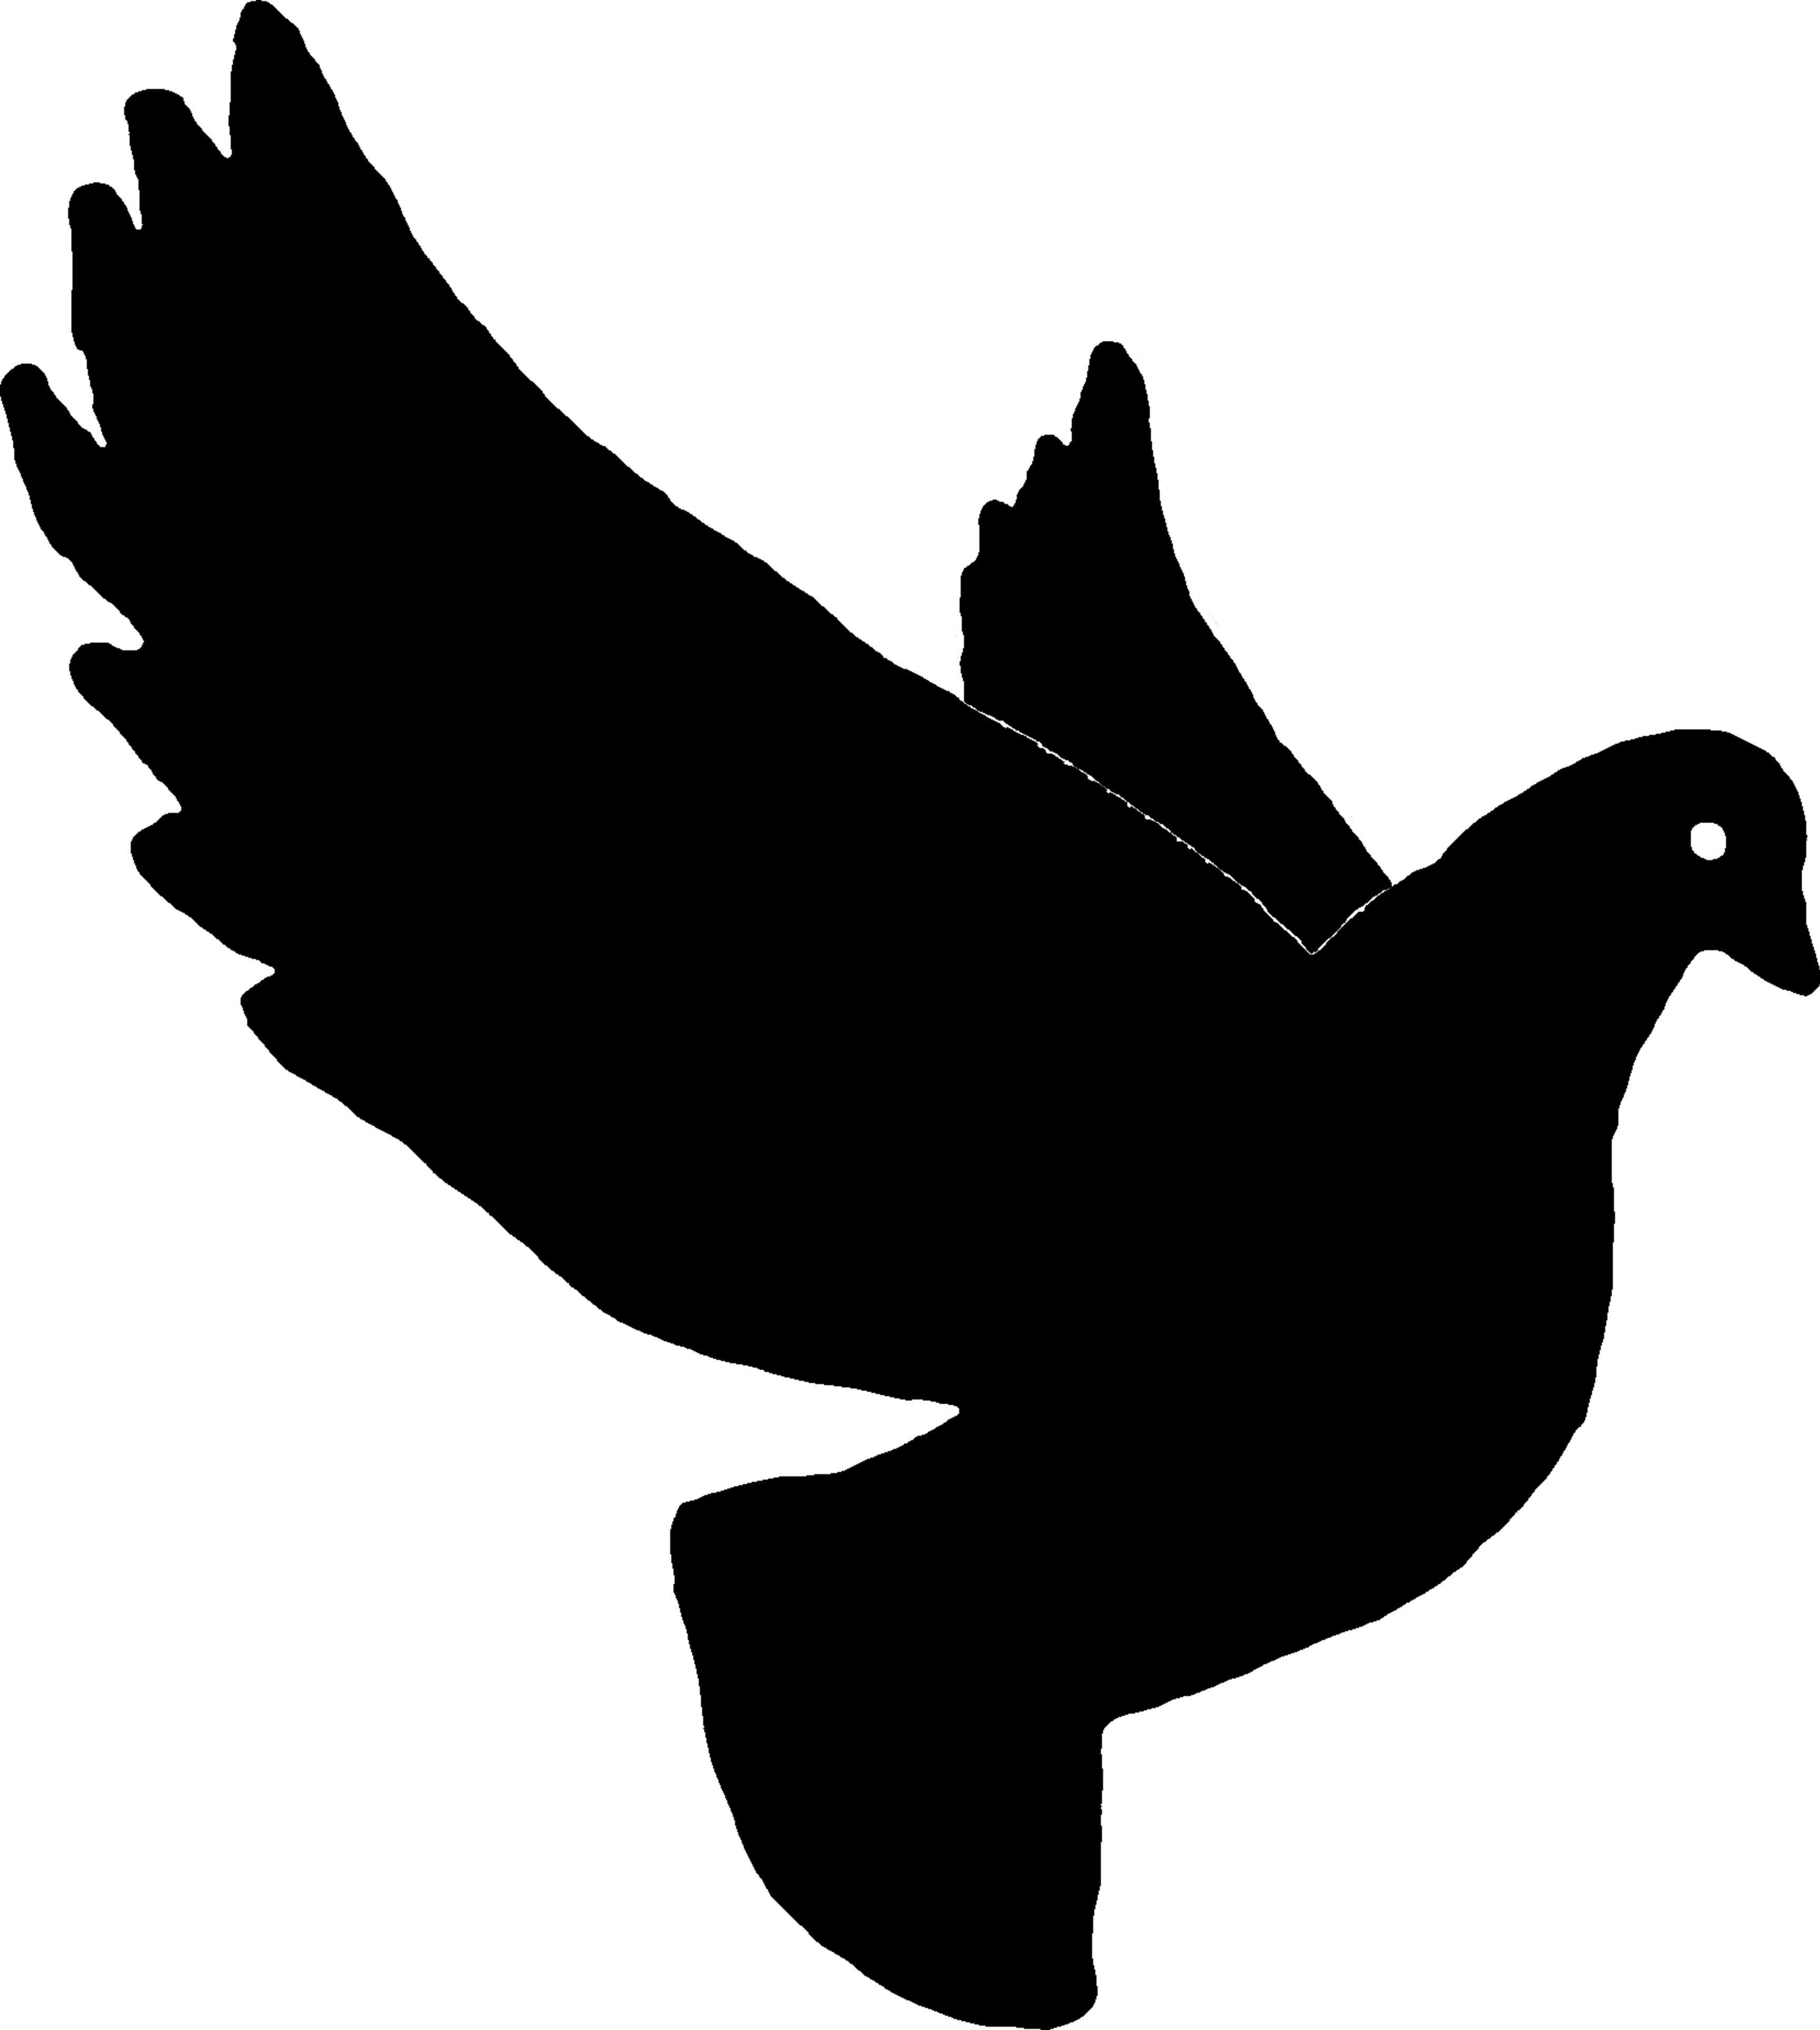
\includegraphics[width=0.5\textwidth]{pigeon.pdf}
		\\ 
		\vspace{\stretch{0.618}}
		jurajholub1@gmail.com
	\end{center}
\end{titlepage}

\begin{multicols}{2}
\tableofcontents
\end{multicols}

\newpage

\begin{Large}\renewcommand\guitarPreAccord{\normalsize\strut}

%%%%%%%%%%%%%% STALE OMSOVE SPEVY
\section{Stále omšové spevy}

\begin{multicols}{2}
\begin{minipage}{\textwidth}
\subsection{Otče náš (veríme ti)}
\begin{guitar}
	\textit{CAPO 2}\\
	/:[F]Otče náš veríme ti.
	[Dmi]Otče nás ponúkame ti.
	[B]Otče náš naše ruky pre [C] bratov.:/
	
	\textit{Medzihra+hovorený Otče náš 
		2x F,Dmi,B,C}
	
	/:[F]Otče nás veríme ti .
	[Dmi]Otče náš ponúkame ti.
	[B]Otče náš naše srdcia pre [C] bratov.:/
\end{guitar}
\end{minipage}

\begin{minipage}{\textwidth}
\subsection{Agnus Dei (Baránok Boží )}
\begin{guitar}
	/:[Emi]Agnus De[C]i, qui tollis peccata [D]mundi, 
	miserere [Emi]nobis:/
	\\
	[G]Agnus [Ami]Dei, qui tollis peccata [G]mundi, 
	dona nobis [D]pacem, dona nobis [C]pacem,
	dona nobis [Emi]pacem.
\end{guitar}
\end{minipage}
\end{multicols}

\begin{multicols}{2}
\begin{minipage}{\textwidth}
\subsection{Nesieme, Pane, chlieb a víno}
\begin{guitar}
	N[Dmi]esieme, Pane, chlieb a [C]víno.
	N[Ami]esieme celý život [Dmi]náš.
	N[Dmi]esieme, Pane, chlieb a [C]víno
	a[Ami] hľadáme Tvoju [Dmi]tvár, Tvoju [C]tvár,
	T[Ami]voju svätú [Dmi]tvár.
\end{guitar}
\end{minipage}

\begin{minipage}{\textwidth}
\subsection{Svätý, svätý, svätý}
\begin{guitar}
	[A]Svätý, svätý, [D]svätý, svätý [A]Pán Boh [Hmi]všetkých [E]sve[A]tov.
	Plné sú [D]nebesia i zem [A]Tvojej [Hmi]slá[E]vy[A].
	Ho[F]san[G]na, ho[A]sanna, ho[G]sanna na [D]výsos[E]tiach!
	[A]Požehnaný, [D]ktorý prichádza [A]v mene [Hmi]Pá[E]no[A]vom.
	Ho[F]san[G]na, ho[A]sanna, ho[F]sanna na [G]výsos[A]tiach!
\end{guitar}
\end{minipage}
\end{multicols}

\newpage
%%%%%%%%%%%%%% CHVALY

\begin{minipage}{\textwidth}
\section{Chvály}
\subsection{Bližšie}
\textit{CAPO 3}
\begin{multicols*}{2}
\begin{guitar}	
	Tvo[Em]ja láska vzala mi [Dsus]dych
	a zmenila [G]môj svet,
	zmenila [C]môj svet.
	\\
	L[Em]en na tom zál[Dsus]eží
	byť s Tebou [G]navždy,
	byť s Tebou [C]navždy.
	\\
	R: [G]Stále bližšie k Tebe [D]kráčať,
	v Tvojej hĺbke sa roz[Em]plývať,
	ja túžim poznať [C]viac,
	Teba poznať [G]viac.
	\columnbreak
	Tvoja láska zmysel [D]dáva
	a všetko preko[Em]náva,
	ja túžim poznať [C]viac,
	Teba poznať [Am]viac[G D].
	Teba poznať [Am]viac[G D].
	\\
	Prechod:
	[C]Woah, [G]woah,
	[Dsus]Tvoja láska [Em]vznešená je.
	Woah, woah,
	Tvoja láska láme.
\end{guitar}
\end{multicols*}
\end{minipage}

\begin{minipage}{\textwidth}
\subsection{Boh je tak blízko nás}
\begin{multicols}{2}
\begin{guitar}
	PREDOHRA: 
	Dm, C, Am7, B, 
	Dm, C, Am7, Dm
	\\
	/:Boh je tak [Dm]blízko [C]nás, 
	Boh je tak [Am7]blízko [B]nás, 
	Boh je tak [Dm]blízko [C]nás, 
	[Am7]Boh je v [Dm]nás.:/ 
	\\
	/:Ty si ten [F]dar od Otca [C]nám, 
	Ty si tá [Gm]láska, čo prišla k [Dm]nám, 
	Ty si ma [B]z hriechu vykúpiť [C]chcel
	– [Am7]Eman[Dm]uel.:/
	\\
	DOHRA: 
	F, C, Gm, Dm, Bb, 
	C, Am7, G, Dm
\end{guitar}
\end{multicols}
\end{minipage}

\begin{minipage}{\textwidth}
\begin{multicols}{2}
\subsection{Vyvyšujem Teba Pane}
\begin{guitar}	
	[C]Vyvyšujem Teba [G]Pane 
	nad týmto [F]dňom,
	[C]vyvyšujem Teba [G]Pane 
	nad každým[F] človekom, 
	[C]vyvyšujem Teba [G]Pane 
	nad všetkým,[F] čo stvorené je,
	[C]vyvyšujem Teba [G]Pane
 nad svojím[F] životom.
	\\
	[C]Vyvyšujem Tvoje [G]meno 
	nad každé [F]meno (4x) 
\end{guitar}

\subsection{Tebe patrí chvála}
\begin{guitar}	
	\textit{CAPO 2}\\
	/:[D]Tebe patrí [G] chvála, 
	česť a [Hmi] sláva,
	pozdvi [Ami] hnime svoje [C] ruky 
	a [D] chváľme Sväté meno.:/
	\\
	Lebo Ty si [G] Pán, 
	veľké veci robíš [Emi] nám, 
	nikto nie je ako [C] Ty, 
	[Ami] nikto [D] nie je ako Ty.	 
\end{guitar}
\end{multicols}
\end{minipage}

\begin{minipage}{\textwidth}
\subsection{Kríž je znakom spásy}
\begin{multicols}{2}
\begin{guitar}
	R: [C]Kríž je znakom [Emi]spásy, 
	[F]kríž ten dreve[G]ný,
	[C]Kristom nesený [Emi]z lásky, 
	[F]krvou zmáča[G]ný za [C]nás.
	\\
	1.[C]Sám si Pane [Emi]znášal, 
	ť[F]archu našich ví[G]n.
	[C]Sám si sa od[Emi]dával 
	[F]z lásky pod svoj [G]kríí[C]-íž.
	\\
	2. [C]Pozri, Pane, hľa [Emi]tu 
	n[F]a mňa úbo[G]hého,
	[C]pomôž znášať ť[Emi]archu 
	k[F]ríža tak ť[G]ažké[C]ho.
	\\
	3. [C]Chcem aj ja niesť [Emi]svoj kríž,
	ť[F]archu svojich [G]vín.
	[C]Krista vždy nasle[Emi]dovať, 
	[F]chcem ísť stále [G]s Níí[C]-ím.
\end{guitar}
\end{multicols}
\end{minipage}

\begin{minipage}{\textwidth}
\subsection{Aj keby nekvitol fík}
\textit{CAPO 2}
\begin{multicols*}{2}
\begin{guitar}	
	1.Aj keby nekvitol [Em] fík,
	aj keby [C]nerodila zem,
	aj keby [Am]nebesá nedoniesli [G]svetlo v nové [H7]ráno.
	A aj keď [Em]polia zlyhajú
	a sýpky [C]prázdne zostanú,
	aj keď [Am]všetko vôkol [G]volá, že Boh [H7]nie je.
	\\
	2.Keď blízky [Em]priateľ opustí,
	a je tak ť[C]ažké odpustiť
	keď sa [Am]múry v mojom [G]vnútri zrazu [H7]rúcajú
	keď sa zdá, ž[Em]e to neskončí,
	slzy sa [C]tlačia do očí
	viem, že [Am]stojíš blízko [G]tých, čo v Teba [H7]dúfajú.
	\columnbreak
	R: 
	Áno [G]práve vtedy pozdvihnem svoj hlas
	a [D]budem spievať chvály.
	Uprostred [C]trápení, uprostred [Am]súžení 
	[H7]Ježiš je Pán.
	Áno [G]práve vtedy pozdvihnem svoj hlas
	a [D]budem spievať chvály.
	[C]Lebo ve[Am]rím, v [C]Neho ve[Am]rím.
	( Aj keby nekvitol [Em]fík )
\end{guitar}
\end{multicols*}
\end{minipage}

\begin{minipage}{\textwidth}
\subsection{Ty si Pánom}
\begin{guitar}
	[G]Ty si Pánom (Ty si Pánom), 
	[D]Ty si Kráľom (Ty si Kráľom),
	[Emi] Ó Kráľom je [C]Boo-[D]oh.
	\\
	/: P[G]ozdvihnime svoje srdcia,
	[D]pozdvihnime svoje dlane, aleluja
	[Emi]postavme sa pred tvár Pána 
	a velebme [C]Hoo-[D]oo. :/
\end{guitar}
\end{minipage}

\begin{minipage}{\textwidth}
\subsection{Až do konca dní}
\begin{multicols*}{2}
\begin{guitar}	
	1.[C]Dnes dávaš [D]všetko čo [Emi]máš.
	[C]Našiel si [D]lásku a [G]tak ju stráž.
	[C]Boh klope [D]na dvere, kým svet [Emi]spí,
	On aj v noci [Ami]bdie 
	a [C]dnes aj ty bdieš s [D]Ním.
	\\
	2.[C]Láska je [D] úsmev a [Emi]plač.
	[C]Smútok a [D]strach náhle [G]zmýva dážď.
	[C]Cítiš, že [D]Boh je tak [Emi]blízko nás,
	Cítiš, že s [Ami]Ním 
	si tak [C]stále viac [D]svoj.
	\\
	3.[C]Vždy príde [D]otázok [Emi]pár,
	[C] čo trápia [D]srdce a [G]trápia tvár.
	[C]Vieš, že ťa [D]nezlomia, [Emi]kým si s Ním, 
	Neboj sa [Ami] ísť, On [C]vie čo s [D]tým.
	\columnbreak
	Boh ti [C]práve dal,
	to [Hmi]znamenie tých nových [Ami]dní,
	[C]krásnych [D]dní.
	\\
	R: Až do konca [C]dní, On [D]chráni ťa [Emi]láskou.
	Dnes ti vrátil [C]raj, tak ho [D]vnútri [G]maj.
	Až do konca [C]dní, ma k [D] človeku [Emi]blízko.
	S Ním nikdy nie si [Ami]sám, [C]až do konca [D]dní.
\end{guitar}
\end{multicols*}
\end{minipage}

\begin{minipage}{\textwidth}
\subsection{Aj keď Ťa nevidím}
\textit{CAPO 1}
\begin{multicols*}{2}
\begin{guitar}	
	1. Aj keď Ťa [C]nevidím, viem, že si tu.
	Aj keď Ťa [Ami]necítim, mám istotu.
	V smelej [F]dôve[C]re kráčam [Ami]vo vie[F]re každý [C]deň.
	Aj keď zvádza ma boj so svetom,
	aj keď ne[Ami]vidím hneď víťazstvo.
	V smelej [F]dôve[C]re kráčam [Ami]vo vie[F]re každý [C]deň.
	\\
	R. /: Nemu[Ami]sím zlého sa [Emi]báť :/
	v smelej [F]dôvere k[Dmi]ráčam [G]vo vie[C]re.
	\columnbreak
	2. Aj keď tem[C]nota mi zastrie zrak,
	aj keď ne[Ami]priateľ ma oblieha.
	V smelej [F]dôve[C]re kráčam [Ami]vo vie[F]re každý [C]deň.
	[C]Aj keď ma [C]obkľúči a zovrie strach,
	Ježiš vždy [Ami]víťazí, mňa má v rukách.
	V smelej [F]dôve[C]re kráčam [Ami]vo vie[F]re každý [C]deň.
\end{guitar}
\end{multicols*}
\end{minipage}

\begin{minipage}{\textwidth}
\subsection{Živý je Pán}
\begin{multicols*}{2}
\begin{guitar}	
	R. /: Ž[Emi]ivý je [A]Pán, ž[D]ivý je [Hmi]Pán, 
	ž[Emi]ivý je [A]Pán na veky [D]vekov. :/
	\\
	1. L[Emi]ebo Pán tak [A]miloval svet, ž[D]e Syn[Hmi]a svojho,
	[Emi]jednorode[A]ného za nás [D]dal.
	[Emi]Aby každý, [A]kto uverí v [D]Neho, nezahy[Hmi]nul, 
	[Emi]ale mal s Ním ž[A]ivot večný [D]v nebi.
	\columnbreak
	2. [Emi]Ak sa niekto [A]nenarodí [D]z vody a [Hmi]z Ducha,
	[Emi]nemôže vojsť [A]do kráľovstva [D]jeho.
	[Emi]Iste nikto [A]s ním nevojde [D]do Božej slá[Hmi]vy, 
	[Emi]ak sa z Boha [A]znova nena[D]rodí.
\end{guitar}
\end{multicols*}
\end{minipage}

\begin{minipage}{\textwidth}
\subsection{Ty si jediný Boh}
\begin{multicols*}{2}
\begin{guitar}	
	Ty si [E]jediný Boh
	[A2]prvý a posledný.
	Nikdy [A]nebol a nebude viacej,
	nikto [E]ako si Ty.
	\\
	[A2]Ty máš [E]najväčšiu moc,
	Ty si z[A2]vrchovaný.
	nikdy [A]nebol a nebude viacej,
	nikto [E]ako si Ty.
	\columnbreak
	R:
	[A2]Si [E]najväčší vo svojej sile.
	[A2]najväčší vo svojej moci.
	[A]Hrozný si vo svojom hneve.
	[E]najväčší vo svojom [A2]milovaní.
	\\
	[E]Svätý vo svojich skutkoch,
	[A2]múdry a dokonalý.
	Nikdy [A]nebol a nebude viacej,
	nikto [E]ako si Ty.
\end{guitar}
\end{multicols*}
\end{minipage}

\begin{minipage}{\textwidth}
\subsection{Privítajme Pána v tomto chráme}
\begin{multicols*}{2}
\begin{guitar}	
	[G]Všade tam, kde sú ľ[D]udia zíde[G]ní
	v mene Ježiš, v [D]láske zjednote[G]ní.
	[Ami]Práve tam Boh [Emi]zasľúbil, ž[C]e bude prítom[G]ný
	[Ami]dnes viem, že [Hmi]náš Boh je 
	[C]na tomto [D]mieste prítomný.
	
	R: /:[C]Privítajme Pána v [G]tomto chráme
	[D]nech ho Božia sláva [G]naplní
	[C]Svojmu Bohu spieva[G]me a hráme
	[D]pieseň spase[G]ných.:/
\end{guitar}
\end{multicols*}
\end{minipage}

\newpage
%%%%%%%%%%%%%% ČEK REPABLIK

\begin{minipage}{\textwidth}
\section{České chvály}
\subsection{Svorni jsme}
\begin{multicols}{2}
\begin{guitar}
	1. Svorni [Emi]jsme v jednom Duchu, 
	vede nás jeden Pán,
	svorni [Ami]jsme v jednom Duchu, 
	vede [Emi]nás jeden Pán.
	S modlit[Ami]bou zříme den, 
	kdy rozkol [Emi]bude překonán.
	\\
	2. Půjdeme [Emi]ruku v ruce, 
	půjdeme k lidem všem,
	půjde[Ami]me ruku v ruce, 
	půjde[Emi]me k lidem všem.
	Společ[Ami]ně rozhlásíme, 
	že Bůh [Emi]přišel v tuto zem.
	\columnbreak
	3. Každý chval [Emi]Boha Otce, 
	od nějž život pochází,
	každý [Ami]chval Syna Jeho, 
	v němž vše [Emi]smysl nachází
	a kaž[Ami]dý chval Dar Ducha, 
	jenž svor[Emi]nosti předchází.
	\\
	R.: Pozna[C]jí nás po lásce, 
	křesťa[Emi]ny, křesťa[Ami]ny,
	Ano, [Emi]po lásce po[C]znají křesťa[Emi]ny.
\end{guitar}
\end{multicols}
\end{minipage}

\begin{minipage}{\textwidth}
\begin{multicols}{2}
\subsection{Duchu Svatý, přijď (sestup mezi nás)}
\begin{guitar}	
	D[Emi]uchu Svatý příď[A], sestup [EMi]mezi nás[A],
	mz Tě [C]voláme[D], probuď nás[Emi].
	\\
	R. Vše co [C]mám, s radostí[D], odevz[Emi]dá[Hmi]vam,
	Vše co [C]jsem, budiž [D]Tvé, jsi můj [Emi]Pán.
\end{guitar}

\subsection{Hle, stojím u dveří}
\begin{guitar}	
	Hle [Dmi]stojím u dveří a tluču, [C]pusť mě [Dmi]dál [C].
	[Gmi]Stojím u dveří a toužím s Tebou být.
	[Dmi]Stojím u dveří a tluču, [C]praví [Dmi]Pán[C].
\end{guitar}

\columnbreak

\subsection{Bůh je síla má}
\begin{guitar}
	[Emi]Bůh je síla má [C]i vojska [D]mého,
	[Emi]On působí [C]volnou cestou [D]mou,
	[Emi]neboť dal mi šťít [C]spasení své[D]ho
	a [Emi]dobrotivost Jeho [C]zvelebila [D]mne.
	\\
	R: /:[G]Neboť kdo je Bohem [C]kromě Hospo[D]dina
	[Emi]A kdo je skálou kromě [C]Boha naše[D]ho.:/
\end{guitar}
\end{multicols}
\end{minipage}

\newpage
%%%%%%%%%%%%%% RIEKA ZIVOTA

\begin{minipage}{\textwidth}
\section{Rieka života}
\subsection{Nad celou zemou}
\textit{CAPO 2}
\begin{multicols*}{2}
\begin{guitar}	
	1.[G]Nad ce[D]lou ze[C]mou, Pán [D]od vek[G]ov,
	nad k[D]aždým vr[C]chom každou [D]doli[G]nou.
	No mojou [D]túž[C]bou Otče [D]je[Ami]dinou,
	je aby [C]vládol[D] sám Syn [G]Tvoj.
	\\
	R:[G] Ó [D]vládni [C]mi, vlád[D]ni s mo[G]cou,
	v čase[D] chvíľ ťaž[C]kých,v rokoch [D] úspeš[G]ných.
	Len[D] Ty si [C]Pán nad [D]tým čo [Emi]mám,
	tak prosím [C]príď a[D] vládni [G]mi.
	\columnbreak
	2. [G]Celým [D]srdcom c[C]hcem, celou [D]mysľou [G]tiež 
	sa [D]Ti podo[C]bať, Bože [D]nádher[G]ný, 
	pre mňa [D]vzácny [C]si v svete [D]je[Ami]diný, 
	tak prosím [C]príď a [D]vládni [G]mi.
	\\
	R: + /:[Emi]Tak prosím [C]príď a [D]vládni [G]mi:/
\end{guitar}
\end{multicols*}
\end{minipage}

\begin{minipage}{\textwidth}
\subsection{Dnes pieseň hrám}
\textit{CAPO 2}
\begin{multicols*}{2}
\begin{guitar}	
	[D]Dnes [A]pieseň [Hmi]hrám a [A]nie som [G]sám, 
	Tebe [D]Ježiš môj [A]Majster.
	[D]A [A]stále [Hmi]viac Ťa [A]túžim [G]mať 
	Ty si [D]najhlbšou [A]túžbou.
	\\
	[Emi]Nech tečie rieka Tvojho [Hmi] života v [A]nás,
	[Emi]chcel by som prežiť dnes Tvoj [A]vodopád.
	[Emi]Daj sa mi napiť z Tvojho [Hmi]prameňa [A]krás,
	[G]znova chcem v [D] úžase [F#mi]stáť[A].
	\columnbreak
	Nechcem bez Teba [D] žiť,
	ááá[F#mi]aáááá[G]aáááá
	[G]Nechcem bez Teba [A] žiť.
\end{guitar}
\end{multicols*}
\end{minipage}

\begin{minipage}{\textwidth}
\subsection{Poď, teraz je čas}
\begin{multicols*}{2}
\begin{guitar}
	[D]Poď, teraz je čas vzdať [G]chvá[D]lu
	[A]Poď, srdce svoje mu s [Emi]láskou [G]daj
	[D]Poď, taký, aký si, [G]chváľ [D]ho
	[A]Poď, predstúp pred kráľa, [Emi]príjme [G] ťa
	[D]Tak poď.
	\columnbreak
	/: [G]Každý jazyk v ten deň vyzná[D], Ty si Pán,
	[G]Každý Ti raz úctu [D]vzdá
	[G]Tým, čo teraz s láskou Ťa [Hmi]hľadajú,
	[Emi]Ty poklad vzácny [A]dáš :/
	[D]Poď.
\end{guitar}
\end{multicols*}
\end{minipage}


\begin{minipage}{\textwidth}
\subsection{Srdce chvály}
\begin{multicols}{2}
\begin{guitar}	
	1. [D]Hudba dohráva [A], všetko stíši [Emi]sa. 
	A ja prichádz[A]am. [D]Priniesť niečo snáď [A],
	čo pravú cenu [Emi]má , čo by si mal [A]rád.
	\\
	R1: [Emi]Viac ako [D]pieseň ti [A]dám, 
	lebo to čo žiadaš. 
	[Emi]Nie je len [D]pieseň sam[A]a, 
	[Emi]ak niečo [D]iné sa z[A]dá.
	Ty vieš čo je pravda, 
	[Emi]ty vidíš, č[D]o v srdci [A]mám.
	\\
	2. Ne[D]konečný k[A]ráľ, nik nevysloví[Emi], 
	čo ti patriť [A]má. 
	Aj[D] keď slabý s[A]om, všetko to čo mám[Emi],
	každý dych je tv[A]oj.
	\\
	R2: [D]Túžim sa vrátiť do [A]srdca chvály, 
	kde si [Emi]jedine ty, [G]jedine ty [A]Ježiš [D].
	Odpusť mi Pane, že [A]neverný som. 
	Si to [Emi]jedine ty, [G]jedine ty [A]Ježiš [D].
\end{guitar}
\end{multicols}
\end{minipage}

\begin{minipage}{\textwidth}
\subsection{Dávam všetko}
\textit{CAPO 2}\\
\begin{multicols}{2}
\begin{guitar}	
	1. [D] Dnes chcel by som Ti [A] dať
	to, čo v srdci [G] mám
	a dávam [A] na ol [Hmi] tár
	k Tvojim [A] nohám kráľov [D] Kráľ.
	\\
	D[D]nes kladiem svoje [A]sny,
	ja sa zriekam svojich [G]práv,
	už nechcem p[A]yšný s[Hmi]táť,
	chcem no[A]vý život [D]mať.
	\\
	R. /: [Hmi] Dáá [A] vam [D] všetko,
	[G] to čo [D] mám, [Hmi] Tebe, [A] kráľ. [G] :/
	\columnbreak
	2. K[D]eď túto pieseň h[A]rám
	pod krížom stojím [G]sám
	a všetky [A]bohat[Hmi]stvá
	za sme[A]ti pokla[D]dám.
	\\
	Ch[D]cem poznať Teba k[A]ráľ,
	slávu mena, ktoré [G]máš,
	tá radosť [A]neko[Hmi]nčí
	aj keď s[A] Tebou trpieť [D]mám.
\end{guitar}
\end{multicols}
\end{minipage}

\begin{minipage}{\textwidth}
\subsection{Všetko to, čo chcem}
\textit{CAPO 1}\\
\begin{multicols}{2}
\begin{guitar}	
	[G]Všetko to, čo [C]chcem, 
	[D]je byť blízko.
	A č[G]o povedať [C]chcem, 
	[D]je, že ďaku-[Emi]jem,
	Že[D] ľúbiš, ma[C] ľúbiš, jé[D]-jéé (2x)
	\\
	R: Ty si[G] ver-[C]ný 
	[Emi]vo všetkom, čo [D]sľúbiš.
	[G]A ľúbiš ma [C]po všetky [D]dni,
	[G]Stá-[C]le, [Emi]aj s mojimi [D]pádmi ma [C] ľúbiš.
	[G]Ma ľúbiš, ma ľúbiš.
\end{guitar}
\end{multicols}
\end{minipage}

\begin{minipage}{\textwidth}
\subsection{Nádherný Boh}
\textit{CAPO 2}
\begin{multicols*}{3}
\begin{guitar}	
	[C] Úžasný, tak [D] úžasný
	si [G]v láske bez hraníc,
	Tvoj k[C]ríž mi dáva
	[D]milosť sľúb[Emi]enú.
	\\
	Nik [C]nevidel, nik [D]nepočul,
	niet [G]srdca, čo tuší,
	jak [C]slávny je 
	[D]a nádherný Boh [G]môj.
	\\
	[C]Všemocný, tak [D]všemocný,
	zem [G]Tvoju slávu má,
	moc [C]Tvojich diel
	[D]v nej každý rozp[Emi]ozná.
	\columnbreak
	Krá[C]sa Tvojho [D]kráľovstva
	spev [G]môjmu srdcu dá,
	tak [C]zázračný,
	[D]tak zázračný Boh [G]si.
	\\
	R:
	Nádherný [C]Boh, Ťa [D] ľúbim,
	nádherný [C]Boh, ja Ťa [D]ctím,
	nádherný [C]Boh, nech [D]pieseň 
	[G]znie.
	\columnbreak
	Dal [C]uzrieť si mi
	všetky [D]zázraky v nás,
	tou [C]láskou si získal [D]ma,
	veď [C]nič na zemi
	sa Ti v [D]kráse nevyrov[G]ná.
	\\
	Mne v [C]duši pieseň [D]znie,
	mne v [C]duši pieseň [D]znie,
	mne v [C]duši pieseň [D]znie,
	nádherný [G]Boh.
\end{guitar}
\end{multicols*}
\end{minipage}

\begin{minipage}{\textwidth}
\subsection{Môj Ježiš, si spásou}
\textit{CAPO 1}
\begin{multicols*}{2}
\begin{guitar}	
	1.[A]Môj Ježiš, [E]si Spásou.
	[F#]Pán nie je [E]nik ako [D]Ty.
	Chcem každý[A] čas,
	[D]tak ako dne[A]s.
	len Teba chváliť
	[G]Pán [D]môj a [E]Kráľ.
	\\
	2.[A]Môj Majster, [E]si Štítom.
	[F#]záchrancom si, [E]Pokoj [D]môj.
	Všetko čo [A]viem,
	[D]všetko čo má[A]m.
	Tebe dávam,
	[G]Pán [D]môj a [E]rád.
	\columnbreak
	R:[A]Sám si Boh môj, celá [D]zem nech [E]vidí,
	že [A]sláva a moc majes[D]tát Ti pat[E]rí.
	[A]Hory pred trónom sa s[D]kláňajú
	a Ty [E]sám [D]vládneš [E]slávne.
	
	[A]Spievam Ti rád, veď s[D]i Pán môj [E]a Kráľ,
	[A]naveky chcem stáť, Teba s[D]tále mať rá[E]d.
	[A]Nič nie je viac ako [D]láska čo da[E]l si [A]nám.
\end{guitar}
\end{multicols*}
\end{minipage}

\begin{minipage}{\textwidth}
\subsection{Síl nám pribúda}
\textit{CAPO 3}
\begin{multicols*}{2}
\begin{guitar}	
	/:Síl ná[G]m pribúda, 
	[C]keď na Teba č[G]akáme,
	[C]keď na Teba č[G]akáme,
	[C]keď Ťa čaká[G]me.:/
	\\
	/:Si B[C]oh, môj večný Vládc[D]a,
	ná[C]dej a mocná spá[D]sa.:/
	\columnbreak
	/:Si [G]svätý, nekonečný [C]Kráľ,
	si stále živý [Emi]Boh,
	Ty neustávaš, ty [C]ne - [D]u - [C]sí - [D]naš.
	[G]Ty sám ochrániš malič[C]kých,
	potešíš plačú[Emi]cich,
	na krídlach orlích ,
	k [C]výš[D]kam [C]dví[D]haš [G]nás.:/
\end{guitar}
\end{multicols*}
\end{minipage}

\begin{minipage}{\textwidth}
\subsection{Zvelebený Pán}
\textit{CAPO 2}
\begin{multicols*}{2}
\begin{guitar}	
	1. [G]Zvele[D]bený buď, 
	tam kde [Emi]kraj medom [C]oplýva.
	Tam, kde [G]rieky vždy [D]hojné sú,
	[Emi]Zvelebený [C]Pán.
	[G]Zvele[D]bený buď, 
	aj keď [Emi]v púšti sa na[C]chádzam.
	Aj keď [G]kráčam sám v [D]pustinách,
	[Emi]Zvelebený [C]Pán.
	\\
	R1:[G]Každú milosť, č[D]o mi dávaš,
	[Emi]vyspievam [C]rád.
	[G]Aj keď tma [D]ma obopína,
	[Emi]ja zavo[C]lám.
	\\
	R2: Zvelebený [G]buď, Pane [D]náš,
	zvelebený [Emi]Pán[C],
	Zvelebený [G]buď, Pane [D]náš,
	požehnané, [Emi]slávne [D]meno [C]máš.
	\columnbreak
	2. [G]Zvele[D]bený buď, 
	keď ma [Emi]lúč slnka zo[C]hrieva.
	Keď je [G]svet krásny, [D]bez tieňa.
	[Emi]Zvelebený [C]Pán.
	[G]Zvele[D]bený buď, 
	aj na [Emi]púti, čo ť[C]ažká je.
	Aj keď [G]obetu [D]prinášam.
	[Emi]Zvelebený [C]Pán.
	\\
	Ref.1 + (2x) Ref.2
	4x /: G D Emi C :/ C
	\\
	3. [G]Zvele[D]bený buď, 
	aj na [Emi]púti, čo ť[C]ažká je.
	Aj keď [G]obetu prináš[D]am, 
	[Emi]Zvelebený [C]Pán.
	/:Máš [G]právo dať aj [D]vziať, 
	máš [Emi]právo dať aj [C]vziať
	Ja [G]stále spievam [D]rád, 
	Z[Emi]velebený [C]Pán.:/ + 2x Ref.2
\end{guitar}
\end{multicols*}
\end{minipage}

\begin{minipage}{\textwidth}
\subsection{Vládca}
\textit{CAPO 2}
\begin{multicols*}{2}
\begin{guitar}	
	[C]Každý z nás dúfa [G]v súcit 
	a bezhraničnú[Emi] lásku.
	Ó, [D]Pane, zmiluj s[C]a.
	[C]Každý z nás túži[G] prijímať 
	milosť odp[Emi]ustenia.
	[D]A nádej spás[C]y[D C D].
	\\
	R: [G]Vládca, vrchmi môže [D]hýbať,
	môj Boh je[C] najmocnejší[G], 
	má moc [Emi]zachrániť [D]nás.
	[G]Víťaz, pôvod večnej [D]spásy
	porazil [C]smrť, z hrobu v[G]stal,
	Ježiš [Emi]víťazne [D]vstal.
	\columnbreak
	[C]Biedny som Ty ma [G]prijímaš 
	všetok môj strach [Emi]a pády.
	Ó, [D]Kriste zmiluj [C]sa.
	[C]Za Tebou túžim [G]kráčať 
	si moja pevná[Emi] nádej,
	[D]dnes sa Ti dáv[C]am[D C D].
	\\
	2xRef.
	\\
	/:[C]Zažiar svetlom, 
	[G]nech Ťa svet [D]vidí, Spievaj, 
	[C]Tebe sláva, 
	[G]Kráľ môj víťaz[D]ný, Ježiš.:/ + Ref.
\end{guitar}
\end{multicols*}
\end{minipage}

\begin{minipage}{\textwidth}
\subsection{Daj mi výhľad}
\begin{multicols*}{2}
\begin{guitar}	
	Teba, [C]Bože môj, hľadám a [G]vyzerám
	daj mi [F]výhľad [Am]odkiaľ vidíš [G]svet.
	Len Ty, [C]Bože môj, si mojou [G]záchranou
	daj mi [F]múdrosť, [Am]Ty vieš čo robiť [G]mám.
	\\
	Teba, [C]Bože môj, hľadám a [G]vyzerám
	daj mi [F]výhľad [Am]odkiaľ vidíš [G]svet.
	Len Ty, [C]Bože môj, si mojou [G]záchranou
	daj mi [F]múdrosť, [Am]Ty vieš kam kráčať [G]mám.
	\columnbreak
	Zo všet[F]kých síl [Dm]Teba [G]len
	nave[F]ky nech [Dm]milu[G]jem
	Si mojou [F]skalou, [Dm]si môj [G]Pán
	od [C]vekov navždy [F]nech Teba [G]milu[C]jem.
	\\
	Ale[F]luja, [Dm]kraľuj [G]nám
	Ale[F]luja, [Dm]kraľuj [G]nám
	Ale[F]luja, [Dm]kraľuj [G]nám,
	si [C]Kráľom nave[F]ky, ale[G]lu[C]ja
\end{guitar}
\end{multicols*}
\end{minipage}

\newpage
%%%%%%%%%%%%%% ESPE
\section{EsPé}

\begin{minipage}{\textwidth}
\subsection{Pre Teba áno}
\begin{multicols}{2}
	\begin{guitar}
		\textit{CAPO 5}
		[C]Nevinný si, odsúdia ťa, [G]vieš
		o ranách, ktoré dotknú sa ťa, [C]vieš,
		prebodnú a vysmejú ťa, [G]vieš,
		poznáš nás a predsa ideš [C]vpred...
		Opustený dávaš všetko, [G]vieš,
		krv a voda z teba musí [C]tiecť,
		výdychom mi dych navraciaš [G]späť,
		poznáš ma a predsa šepkáš...
		\\
		Ref.1: (Za teba) [C] Áno, za teba [D]pôjdem.
		Hoden si [Emi]prijať, čo strácam,
		svoj život za tvoj [G]dám.
		\\
		[C]Kráčam s tebou, odsúdia ma, [G]viem
		o ranách, ktoré dotknú sa ma, [C]viem,
		prebodnú a vysmejú ma, [G]viem,
		poznám ich a predsa idem[C]...
		Opustený dávam všetko, [G]viem,
		krv a voda aj zo mňa musí [C]tiecť,
		ľúbiť ťa, cez ľudí vôkol [G]chcem,
		keď nevládzem, ma dvíha tvoje...
		\\
		Ref.1: (Za teba) [C] Áno, za teba [D]pôjdem!
		Hoden si [Emi]prijať, čo strácam,
		svoj život za tvoj [G]dám.
		\\
		Bridge: [C]Moje ústa máš – [D]hovor, po čom túžiš.
		[Emi]Moje nohy máš – [G]kráčaj, kam len túžiš.
		[C]Moje ruky máš – [D]konaj to, čo túžiš.
		[Emi]Moje srdce máš – [G]miluj, ako vieš len ty.
		\\
		Ref.2: (Pre teba) [C] Áno, pošli ma, [D]pôjdem!
		Ohlásim [Emi]zajatým slobodu, zlomeným nádej [G]dám .
	\end{guitar}
\end{multicols}
\end{minipage}

\begin{minipage}{\textwidth}
\subsection{Buď odvážny}
\textit{CAPO 2}
\begin{multicols}{2}
\begin{guitar}
	1. /:Stále [Emi7] viac Teba hľa [G] dám,
	nechcem [C9] žiť bez Teba.
	Skrze Tvoj [Emi7] kríž znovu vi [G] dím,
	nový [C9] dych si mi dal [D]. :/
	\\
	Ref:
	/: Tak buď [Emi7] odvážny môj Duch
	a [D] ber do ruky zbraň
	a [G] smelo vyzná [C9] vaj,
	že Boh [Emi7] drží nado mnou
	[D] triumfálnu stráž
	a [G]nikdy nepres [C9]tal. :/
	\columnbreak
	2. /:Ja viem Tvoja krv
	v mojich žilách dáva život a smiech.
	Láska Otca, obeť Syna 
	už dávno zlomila hriech. :/
	\\
	Ref.
	\\
	Bridge: /: Veď On je [C9] verný Kráľ [D] ,
	[Emi7] zachováva [D] sľuby, ktoré dal.
	A ja [C9] víťazím [D] ,
	lebo [Emi7] prijímam Spásu, [D] ako Boží dar. :/
	\\
	Ref. + Bridge + Ref.
\end{guitar}
\end{multicols}
\end{minipage}

\begin{minipage}{\textwidth}
\subsection{Na krídlach lásky}
\begin{multicols*}{2}
\begin{guitar}
	[Emi]Voláš ma tam,
	[G]kde tvoja sláva prebýva,
	[D]voláš ma tam,
	[C]kde láska sa neskrýva.
	\\
	[Emi]Silu mi dáš
	[G]aj keď nevládzem,
	[D]len s tebou chcem ísť
	[C]keď strácam už nádej.
	\\
	[G]Oo[Ami]oooo[Emi]oooo[C]oo
	\columnbreak
	[Emi]Na krídlach lásky Pane,
	[G]nesieš ma neprestajne,
	[D]voláš ma do hĺbky,
	[C]preskúmať krásu krás.
	\\
	[Emi]Kým ruky zdvihnuté mám
	[C]ja víťazím,
	[G]kým pohľad na teba mám
	[D]ja mám dosť síl.
\end{guitar}
\end{multicols*}
\end{minipage}

\begin{minipage}{\textwidth}
\subsection{Náš Pán On je kráľov Kráľ}
\begin{guitar}
	[Emi]Náš [C]Pán On je [G]kráľov Kráľ, 
	jeho [D]trón, bude [Emi]na veky stáť, 
	On [C]má všetku [G]vládu a moc, 
	náš [Ami]Pán, On je [Hmi]kráľov [Emi]Kráľ.
\end{guitar}
\end{minipage}

\begin{minipage}{\textwidth}
\subsection{Veríme Ti}
\textit{CAPO 4}
\begin{multicols}{2}
\begin{guitar}
	[Emi]Boh, čo slepým [Hmi]dáva zrak,
	[C]Búra múry predo mnou,
	Búra múry predo mnou.
	\\
	[Emi]Boh, čo hluchým [Hmi]dáva sluch
	[C]Tíši vo mne každý strach,
	Tíši vo mne každý strach.
	\\
	Ref. [Emi]Veríme Ti, [C]veríme Ti,
	[G]Ty si Bohom zázrak[D]ov.
	\\
	[Emi]Boh, čo koná [Hmi]nemožné,
	[C]Robí z nás nové stvorenie
	Robí z nás nové stvorenie
	[Emi]Boh, čo vládne [Hmi]nad smrťou,
	[C]Prúdi v nás svojim životom
	Prúdi sojim životom.
	\\
	Ref.
	\\
	[G]Boh, čo bol a [D]príde zas
	[G]Tá moc, čo Syna vzkrie[Emi]sila
	[C]Boh, čo mŕtvym [D] život dá
	Ty si Bohom [G]zázrakov
	Si Bohom zázrakov
	\\
	Ref.
\end{guitar}
\end{multicols}
\end{minipage}

\begin{minipage}{\textwidth}
\subsection{Náš Boh}
\textit{CAPO 2 (dá sa aj bez)}
\begin{multicols}{2}
\begin{guitar}
	[Emi]Vodu na [C]víno me[G]níš,
	[Emi]otváraš [C]oči sle[G]pým,
	nikto [Ami]nie je ako [D]Ty.
	\\
	[Emi]Zasvietiš [C]v tmách živo[G]tom,
	[Emi]z prachu nás [C]dvíhaš Slo[G]vom,
	nikto [Ami]nie je ako [D]Ty.
	\\
	R: [Emi]Náš Boh je väčší, [C]On je silnejší,
	[G]Pane, si viac než čo [D]tento svet dáva.
	[Emi]Rany nám liečiš, [C]mocný a slávny
	náš [G]Boh, si náš [D]Pán
	\columnbreak
	[Emi]Zasvietiš [C]v tmách živo[G]tom,
	[Emi]z prachu nás [C]dvíhaš Slo[G]vom,
	nikto [Ami]nie je ako [D]Ty. \textit{+ 2x Ref.}
	\\
	/:[Emi]Veď keď náš Boh je za nás
	[C]nemôže vládnuť strach
	[G]keď náš Boh je s nami
	[D]kto môže stáť proti nám?:/ \textit{+ 2x Ref.}
\end{guitar}
\end{multicols}
\end{minipage}

\newpage
%%%%%%%%%%%%%% LCH

\begin{minipage}{\textwidth}
\section{Lamačské chvály}
\begin{multicols}{2}
\subsection{Ovečka / Ja milujem Kráľa a on ľúbi}
\begin{guitar}	
	[D]Som Tvojou ovečkou	
	[A]malou a voňavou	
	č[Hmi]istou a radostnou 
	[G]Tebou ľúbenou.
	\\
	[D]Ja milujem Kráľa a on ľúbi mňa
	[A]ja milujem Kráľa a on ľúbi mňa
	[Hmi]ja milujem Kráľa a on ľúbi [G]mňa.
\end{guitar}
\columnbreak
\subsection{Ty si Boh ktorý vládne}
\begin{guitar}	
	/: Ty si [C]Boh ktorý vládne[G], na [A]nebi[F],  
	Ty si [C]Boh ktorý vládne[G], na [A]zemi[F]. :/ 
	\\
	/: Kto Ťa [C]oslávi[G], kto Ťa [A]vyvýši[F], 
	kto Ti[C] chválu vzdá[F], ak nie[A] my[F]? :/
	\\
	/: Ja Ťa [C]oslávim[G], ja Ťa [A]vyvýšim[F],
	ja Ti ch[C]válu vzdám[F], Jež[A]iš môj[F]. :/
\end{guitar}
\end{multicols}
\end{minipage}

\begin{minipage}{\textwidth}
\subsection{Verný si}
\begin{multicols*}{2}
\begin{guitar}
	1.Vž[C]dy keď vstávam, blízko si,
	K[F]eď si líham, blízko si,
	A[Ami]j keď ťa [G]nevi[F]dím,
	[C]V každom čase, verný si,
	[F]Aj keď som sám, verný si,
	[Ami]Aj keď ťa[G] necí[F]tim,
	\\
	2.[C]V každom čase, verný si,
	[F]Aj keď som sám, verný si,
	[Ami]Aj keď ťa[G] necí[F]tim,
	[C]Keď všetko padá, stály si,
	[F]v každej zmene, stály si,
	[Ami]ja ti [G]ve[F]rím,
	\columnbreak
	R:J[F]a v[G]iem, že si [C]tu,
	[F]Jež[G]iš, ty si [Ami]tu.S tebou Ježiš [Ami]môj
	zvíťa[G]zím, zvíťa[F]zím, zvíťa[C]zím,
	[Ami]Ja vi[G]em, láskou [F]hriech pora[C]zím,
	[Ami]Ja vi[G]em, s tebou [F]zvíťa[C]zím,
	lebo t[F]y si [C]už, z[G]víťaz[F]il
	\\
	Outro:
	Ďa[C]kujem ti pane, 
	za [F]tvoje požehnanie, 
	[Ami] že pri m[G]ne sto[F]jíš,
	Nech[C] tvoja láska pane, 
	sa [F]mojou láskou stane,
	[Ami] ja [G]ti ve[F]rím.
\end{guitar}
\end{multicols*}
\end{minipage}

\begin{minipage}{\textwidth}
\subsection{El Shaddai}
\begin{multicols*}{2}
\begin{guitar}
	[C]Vystačím si sám, [E]tak si vravím,
	ž[Ami]e všetko už mám, [F]cítim sa tým pravým.
	[C]Keď ku tebe prídem a [E]dotkneš sa mi dlaní,
	[Ami]zrazu to vidím, [F]bol som oklamaný.
	\\
	[C]Toľko chvíľ som stratil, 
	[E]vzácnych, pripravených,
	[Ami]cestu som si krátil, [F]keď ma nevideli.
	[C]Bezradne tu stojím, [E]stojím zahanbený,
	[Ami]túžim znovu skákať, byť [F]tebou zachránený.
	\\
	R. /:[C]Ty si ten mocný kráľ,
	[E]El Shaddai, Adonai,
	[Ami]ochranca maličkých,
	[F]zástanca chudobných.:/
	\columnbreak
	Vidíš moju vieru, aj moje pády.
	Nechcem sa rozpínať, 
	chcem byť znovu malý.
	Víťazstvá sú tvoje, sláva ti patrí.
	V tebe sa chcem ukryť pred sebou samý.m
	\\
	Vraciaš mi nádej, prejavuješ priazeň.
	Vylievaš sám seba, 
	až to po mne steká na zem.
	Dotýkaš sa v hĺbke, viac, než to chápem.
	Chrániš mi chrbát, s tebou znovu vládzem.
	\\
	Ref.
	\\
	Ľúbiš ma nežne, nevtieraš sa mi,
	ani nečakáš, kým budeme sami.
	Si stále so mnou a je ti to vzácne.
	Zvádzaš ma, zvádzaš,
	a ja nechal som sa ti zviesť.
\end{guitar}
\end{multicols*}
\end{minipage}

\newpage
%%%%%%%%%%%%%% HEARTBEAT

\begin{minipage}{\textwidth}
\section{Heartbeat}
\subsection{Aleluja}
\textit{CAPO 2}
\begin{multicols*}{3}
\begin{guitar}
	G E D A Woah
		
	[G]Budem chváliť, 
	[E]celým telom,
	[C#]svojim tancom,
	a [A]svojim spevom.
	\\
	[G]Aleluja, [E]aleluja, 
	[D]aleluja [A]znie.
	Poď sloboda, rozprúď ducha
	nech tu radosť neutícha.
	\columnbreak
	[E]A aj nech svet sa rúca
	[A]ja viem, kam kráčať mám
	[E]aj keď sa vody búria
	[A]učíš ma kráčať po vlnách.
	\\
	Voláš ma do tanca
	dávam ti svoju dlaň
	zatváram svoje oči
	otváram srdce dokorán.
	\columnbreak
	[G]Nad každou [A]bolesťou
	nad každým trápe[H]ním
	učíš ma tanco[F#]vať
	počujem, spievaš mi.
\end{guitar}
\end{multicols*}
\end{minipage}

\begin{minipage}{\textwidth}
	\subsection{Verný Boh}
\begin{multicols*}{2}
\begin{guitar}
	[Hmi]Nemôžem [D]prestať [G6]myslieť na teba,
	[Hmi]nemôžem [D]sa ťa [G6] striasť.
	[Hmi]Si ako [D]oheň v mojom [G6]vnútri, 
	čo páli ma,[Hmi D G6] páliš ma.
	\\
	[Hmi] Si [D]všetko, čo [G]chcem,
	[Hmi] si [D]všetko, čo [G]mám,
	[Hmi]aj keď [D]zdá sa, že [G]spíš, 
	ja tvoje meno zavo[C]lám
	proti búrkam, proti t[D]mám.
	\columnbreak
	Si [G]verný Boh a [D]verný kráľ,
	[Emi]dokončíš dielo, [C]ktoré si vo mne začal.
	[G]Verný Boh, [D]verný kráľ, [Emi]nevzdáš sa snov, 
	ktoré si [C]so mnou snívať začal.
	\\
	[G]Ohlásim zo striech,
	[D] že ľúbiš ma a ja ľúbim teba.
	[Emi]Ohlásim zo striech,
	že si [C]verný a verný a verný [G]kráľ.
\end{guitar}
\end{multicols*}
\end{minipage}

\begin{minipage}{\textwidth}
\subsection{Striasam Zo Seba Bohatstvo Tohto Sveta}
\begin{multicols*}{4}
\begin{guitar}
	[D]Striasam zo seba
	[A]bohatstvo tohto sveta
	[G]nech znova vidím Ťa,
	nech [Hmi]znova počujem 
	[A]Tvoj hlas.
	\\
	[D]Oblečiem si chválu
	[A]a zahalím sa do nej
	[Hmi]pravdu vyvýšim
	[G]nič mi nezabráni.
	\\
	[D]Darujem ti slávu
	[A]pôjdem ľahšie bez 
	nej
	[Hmi]lásku vyvýšim
	[G]nič mi nezabráni...
	\columnbreak
	...[D]prísť
	pred Tebou [A]stáť
	[Hmi]Oblečiem si chválu
	[G]a budem uctievať
	\\
	[D]Striasam zo seba
	[F#]bohatstvo tohto sveta
	nech [Hmi]znova vidím Ťa,
	nech [Hmi]znova počujem 
	[A]Tvoj hlas.
	\\
	[D]Svojim spevom 
	a svojim tancom
	[F#]a celým srdcom
	Tebe chválu [Hmi]vzdám,
	Tebe chválu [Emi]vzdám[F#].
	\columnbreak
	[D]Svojim smiechom 
	a svojim plačom
	[F#]a každým dychom
	Tebe chválu [Hmi]vzdám,
	Tebe chválu [Emi]vzdám[F#].
	\\
	[D]Lebo ak budem
	 mlčať,
	[A]kamene budú kričať.
	[Hmi]Slávny, si slávny 
	[G]Kráľ.
	\\
	[D]Lebo ak budem
	mlčať,
	[A]kamene budú kričať.
	[Hmi]Svätý, si svätý [G]Kráľ.
	\columnbreak
	[D]Svojim spevom 
	a svojim tancom
	[Emi]a celým srdcom
	Tebe chválu [D]vzdám,
	Tebe chválu [G]vzdám[A].
	\\
	[D]Svojim smiechom 
	a svojim plačom
	[Emi]a každým dychom
	Tebe chválu [D]vzdám,
	Tebe chválu [G]vzdám[A].
\end{guitar}
\end{multicols*}
\end{minipage}

\begin{minipage}{\textwidth}
\subsection{Vezmi ma}
\begin{multicols*}{2}
\begin{guitar}
	/:[G](Prosím)Vezmi ma na chvíľu z tejto Zeme,
	nechám sa [D]unášať vetrom do vnútrozeme.
	A [Emi]dívať sa na všetko z výšky, zhora,
	chcem [C]zabudnúť, čo bolo dnes a včera.:/
	\\
	/: Na miesta [G]nové, (zaveď ma Kráľ)
	na miesta [D]nepoznané, (zaveď ma Kráľ).
	Aj tie [Emi]zabudnuté, (zaveď ma Kráľ),
	tam, kde [C]moje srdce pre to Tvoje začalo biť.:/
\end{guitar}
\end{multicols*}
\end{minipage}

\newpage
%%%%%%%%%%%%%% RICHARD CANAKY

\begin{minipage}{\textwidth}
\section{Richard Čanaky}
\subsection{Aj keď málo mám síl}
\begin{multicols*}{3}
\begin{guitar}
	[C] Aj keď málo mám síl 
	a [G] cítim sa sám,
	keď [Ami] padám do hriechov, 
	cestu [F] nenachádzam.
	Keď [C] vôkol mňa tieň 
	už [G] rozkladá stan,
	aj keď [Ami] nepriateľ zúri, 
	ja [F] nezaváham.
	\columnbreak
	Svoju záchranu mám, 
	hľadím na kríž,
	skoro zjav sa nám, 
	skoro príď, Ježiš.
	Z prachu dvíhaš ma sám, 
	zmývaš môj hriech,
	znovu cítim, že mám 
	Tvoju nádej aj smer.
	\columnbreak
	Svoje srdce dám pred Tvoj 
	trón,
	život dávam len Tebe, 
	Ježiš, môj Boh.
	Buď mi svetlom dní, 
	keď blúdim v tmách,
	buď mi priateľom, 
	chcem počuť Tvoj hlas,
	chcem počuť Tvoj hlas.	
\end{guitar}
\end{multicols*}
\end{minipage}

\begin{minipage}{\textwidth}
\subsection{Obeta srdca (Túžim priniesť na oltár)}
\begin{multicols*}{3}
\begin{guitar}
	1.[D]Túžim priniesť na ol[G]tár, 
	život č[A]o v sebe [D]mám,
	tvojou láskou zlome[G]ný, 
	chcem ťa [A]chváliť môj [D]Pán.
	Chcem ti vydať práve [G]dnes, 
	každú č[A]asť života[Hmi],
	viem, že prijmeš každý [G]dar, 
	zlome[A]ného srdca[D].
	\columnbreak
	R:
	Povedz čo ti smiem [G]dať, 
	čo p[A]riniesť ti [D]smiem?
	Si môj láskavý Kráľ[G], 
	ja len [A]miznúci tieň[D].
	Ježiš viac nemám slov[G], 
	pieseň [A]doznieva tiež[D],
	aj keď nehodný som[G], 
	chcem ti n[A]iečo priniesť[D].
	Možno len tichý plač, 
	[Emi]len [D]bolesť čo mám[G],
	svoju [Emi]hĺbku [D]srdca ti dám[G], 
	môj [A]láskavý Pán.
	\columnbreak
	2.[D]Kvôli tebe dýchať [G]smiem, 
	môj dlh [A]splatil si [D]sám
	život svoj si za môj [G]dal, 
	bol to [A]víťazný [D]plán.
	Vzal si hanbu z mojich [G]pliec, 
	bol to [A]posledný boj[Hmi], 
	otvoril si bránu ne[G]bies, 
	dnes [A]som iba tvoj[D].
\end{guitar}
\end{multicols*}
\end{minipage}

\begin{minipage}{\textwidth}
\subsection{Jedine s láskou}
\begin{guitar}
	\textit{CAPO 2}
	1.
	[G]Keby mi hlas ako anjela znel, [D]keby som bol prorok veľkých diel,
	[E]keby som aj hory prenášal, [C]bez lásky by som [D]ostal sám.
	
	2.
	[G]Keby som bol múdry ako kráľ, [D]majetok svoj celý rozdával,
	[E]keby som vo svete slávnym bol, [C]bez lásky som iba [D]prázdny kov.
	
	3.
	[G]Keby som v modlitbách stále stál, [D]keby som nad hlavou žiaru mal,
	[E]keby som každý deň v chráme bol, [C]bez lásky som iba /: [D]plný slov :/ (4x)
	
	
	Ref.
	/:[G]Jedine [D]s láskou, [E]jedine [C]s láskou,
	[G]jedine [D]Ježiš Ti [E]dáva, dáva, [C]dáva, [D]lásku, tak [G]poď.:/ 
	
	4.
	[G]Keby som mal v sebe veľa snov, [D]keby som nakŕmil žobrákov,
	[E]keby som celé dni vyhrával, [C]bez lásky je to [D]smiešny bál.
	
	5.
	[G]Keby som zázraky robiť smel, [D]keby som neurobil žiadny hriech,
	[E]keby som na tvári úsmev mal, [C]bez lásky som iba  /: [D]smiešny klaun :/ (4x)
	
	Ref.
\end{guitar}
\end{minipage}

\begin{minipage}{\textwidth}
\subsection{Vznešený}
\begin{guitar}	
	[D]Vznešený tak jemný[G]
	Iba [A]Ty vieš ku nám [D]byť
	Zranení, zlomení[G]
	Bez obáv[A] môžeme [Hmi]prísť
	Ty [A]stále č[G]akáš. [Hmi]Novú [A]nádej nám [G]dáš
	[Hmi]Ty [A]odnímaš [G]hriech. [Hmi]V tichu [A]modlitba [G]znie
\end{guitar}
\end{minipage}

\begin{minipage}{\textwidth}
\subsection{Ty ma nesieš sám}
\begin{multicols*}{2}
\begin{guitar}	
	[G]Ty ma nesieš [C]sám, Tebe [D]veriť s[G]miem.
	Ty mi pomá[C]haš, keď ma [D]láka [Emi]hriech.
	Ty sa [D]dotýkaš [C]hviezd, aj detských [G]sĺz.
	Ty po[D]chopiť vi[C]eš.
	\\
	[G]Tebe ustúp[C]ia, temné [D]mraky [G]s tmou.
	Ty utíš[C]iš, búrky [D]nado [Emi]mnou.
	Tebe [D]nemôže [C]vziať, Tvoju slávu [G]nik,
	ani [D]tvoj majes[C]tát.
	\columnbreak
	[C]Ja chválu Tebe [G]vzdám
	pred iným sa nesklo[D]ním
	Tvoje meno v srdci [Emi]mám
	Tvoje [D]meno vyslo[C]vím!
	\\
	[C]Ja chválu Tebe [G]vzdám
	aby Tvoj Duch prúdil [D]mnou
	aby uzdravený [Emi]bol,
	kto sa [D]skloní pred Te[C]bou!
\end{guitar}
\end{multicols*}
\end{minipage}

\newpage
%%%%%%%%%%%%%% TIMOTHY

\begin{minipage}{\textwidth}
\section{Timothy}
\subsection{Prišli sme ťa vzývať}
\begin{multicols*}{2}
\begin{guitar}	
	1.[D]Do tmy na[A] svet 
	prišlo [G]k nám svetlo sveta.
	[D]Otvor môj[A] zrak nech vi[G]dím
	[D]Krásu lásk[A]y, v ktorej[G] srdce Ti spieva.
	Veď [D]láska a [A]moc Ti pat[G]rí.
	\\
	2.[D]Kráľ všetkých [A]dní 
	a tiež [G]najvyšší vládca.
	[D]Slávnejší [A]nad nebe[G]sá.
	[D]Ponížil [A]sa, prišiel [G]na Zem, čo stvoril,
	[D]vzdal sa slá[A]vy z lásky k [G]nám.
	\columnbreak
	R: Prišli sme Ťa [D]vzývať, 
	prišli sme sa [A]skláňať
	Prišli sme Ti [Hmi]vyznať: Si náš [G]Boh.
	Si dokonalá [D]láska, dokonale [A]svätý,
	dokonale[Hmi] nádherný ku[G] nám.
	/:Ja [A]nemám [D]dosť slov [G]opísať 
	cen[A]u, kto[D]rú Ťa [G]môj hriech stál:/
\end{guitar}
\end{multicols*}
\end{minipage}

\begin{minipage}{\textwidth}
\subsection{Nohy jeleníc}
\begin{multicols}{2}
\begin{guitar}	
	[C]Ty mi dávaš [G]nohy jeleníc
	[Ami]s tebou naberiem [F]denne nových síl.
	[C]S tebou preskočím [G]aj múry trápenia,
	[F]a mojej ceste dáš , [C]pečať víťazstva.
	\\
	Kde nadej zomrela, vzkriesenie zatrúbi
	a hymnu slobody mi do úst položíš,
	nikto už nevezme čo si mi zasľúbil
	zo žalmom na perách zaspávaš v pokoji
\end{guitar}
\end{multicols}
\end{minipage}

\begin{minipage}{\textwidth}
\subsection{Božia láska príd}
\begin{guitar}
	\textit{CAPO 2}
	[C]Božia [F]láska [C]príď, ako [F]mocný [G]oceán .
	\\
	/: [Emi]Prúď cez [Ami]nás [Emi]svojou [Ami]milosťou, 
	Božia [Dmi]lásk[F]a p[G]ríď k [C]nám :/
\end{guitar}
\end{minipage}

\newpage
%%%%%%%%%%%%%% K DUCHU SVATEMU
\section{K Duchu Svätému}

\begin{multicols}{2}
\begin{minipage}{\textwidth}
\subsection{Duchu Svätý príď}
\begin{guitar}
	/:[D]Duchu [A]Svätý p[G]ríď,
	D[D]uchu [G]Svätý [A]príď:/
	\\
	/:Nech [G]zavládne v[D]iera,
	nech z[G]avládne [D]nádej,
	nech z[G]avládne lá[D]ska v [A]nás:/
\end{guitar}
\end{minipage}

\begin{minipage}{\textwidth}
\subsection{Ty si najvyšší, Ty si Pán}
\begin{guitar}
	/:[C]Ty si najvyšší, [Ami]Ty si Pán,
	[F]to, čo mám, Tebe [G]ponúkam.:/
	/:[C]Obnov ma svojím [Ami]Duchom Svätým,
	[F]nech ako Ty [G]stále svietim.:/
\end{guitar}
\end{minipage}
\end{multicols}


\begin{minipage}{\textwidth}
\begin{multicols*}{2}
\subsection{Nech Tvoj Duch preteká}
\begin{guitar}
	Nech Tvoj Duch [C]preteká ako rieka [Ami]mohutná,
	nech Tvoj Duch [F]preteká ako rieka [G]mohutná.
	A rany [C]uzdraví ako rieka [Ami]mohutná,
	a rany [F]uzdraví ako rieka [G]mohutná.
	A bolesť [C]odplaví ako rieka [Ami]mohutná,
	a bolesť [F]odplaví ako rieka [G]mohutná.
	Pokojom [C]naplní ako rieka [Ami]mohutná,
	pokojom [F]naplní ako rieka [G]mohutná.
	Nech zaznie [C]hymna chvál ako rieka 
	[Ami]mohutná,
	nech zaznie [F]hymna chvál ako rieka 
	[G]mohutná.
\end{guitar}
\columnbreak
\subsection{Teraz vchádzaš, Pane}
\begin{guitar}
	\textit{CAPO 3}
	Teraz [D]vchádzaš, Pane
	[A]cez zavreté [F#7]brány
	[Hmi]rany [A]oslá[G]vené
	[F#]Ježiš, [G]víťaz [A]slávny
	\\
	Ty zo[D]stávaš s nami
	[A]zošli svojho [F#7]Ducha
	[Hmi]uzdrav [A]moje [G]srdce
	[F#]daj, nech [G]Tebou [A]dý[h]cha
\end{guitar}
\end{multicols*}
\end{minipage}

\begin{minipage}{\textwidth}
\subsection{Duchu svätý, si tu vítaný}
\begin{multicols*}{3}
\begin{guitar}	
	[D]Nič ma neláka viac
	ako bližšie [G]stáť
	Nič sa nevyrovná
	tomu, čo si nám [D]dal,
	v Tvojej blízkos[G]ti
	\\
	[D]Ja poznám a viem
	Tvoja láska je [G]liek
	v nej slobodný som
	a hanby už [D]niet,
	v Tvojej blízkos[G]ti
	\columnbreak
	[D]Duchu Svätý si tu vítaný,
	príď [G]vtiahni nás
	tam kde [Em]tróniš Ty,
	\\
	Tvoja [D]sláva prichádza dnes
	s túžbou k nám,
	zaplav [G]láskou k Tebe
	naše [Em]srdcia, Kráľ
	\columnbreak
	[D]Nech stále viac pred Tebou
	bázeň mám
	[G]Dnes túžim zažívať,
	aký [Em]dobrý Boh si k nám
\end{guitar}
\end{multicols*}
\end{minipage}

\begin{minipage}{\textwidth}
\subsection{Jak jeleň dychtí za vodou}
\begin{guitar}
	
	R: /:[Emi]Jak [C]jeleň [D]dychtí za vo[Emi]dou
	ja[C] Bože [D]túžim za Te[Emi]bou:/
	\\
	Zošli[Emi]dážď, zošli[C] dážď, dosť[G] bolo su[D]cha.
	Zošli dážď, zošli dážď, Svätého Ducha.
	Zošli dážď, zošli dážď, nové Turíce.
	Zošli dážď, zošli dážď, rozjasaj srdce.
\end{guitar}
\end{minipage}	


\begin{minipage}{\textwidth}
	\subsection{Príď už, príď, Duchu Stvoriteľu}
	\begin{guitar}
		1.[G]Príď už, [D]príď, Duchu [Emi]Stvori[C]teľu, [G]Duchu [D]zmiere[G]nia[D].
		[G]Príď už[D] a premeň ľ[Emi]udstvo [C]celé [G]v nové [D]stvore[G]nia[D].
		\\
		R: [G]Duchu [D]Svätý, [Emi]svojou [Hmi]hmocou [C]v láske [D]obnov [G]nás[D],
		[G]nene[D]chaj nás [Emi]kráčať [Hmi]nocou, [C]osvieť [D]rozum [G]náš[D].
		\\
		2. [G]Prebuď [D]nás svojím [Emi]Duchom [C]Svätým, [G]zažeň [D] temno[G]tu[D].
		[G]Navráť [D]zblúdilých, [Emi]prebuď [C]hluchých, [G] žehnaj [D] živo[G]tu[D].
		\\
		3. [G]Prebuď [D]svedomie [Emi]otupe[C]ných, [G]zbližuj [D]náro[G]dy[D].
		[G]Zavej [D]a priveď [Emi]zotroče[C]ných [G]v ríšu [D]slobo[G]dy[D].
	\end{guitar}
\end{minipage}

\begin{minipage}{\textwidth}
\subsection{Naplň ma Duchom svojím}
\begin{guitar}
	[C]Naplň ma Duchom svo[Ami]jím, [Dmi]naplň ma Duchom svo[G]jím,
	nechcem byť [C]prázd[E]ny [Ami]džbán, plň ma Ty [F]Páá-ne [G]sám.
	[Ami]Naplň ma Duchom svo[Emi]jím, [F]naplň ma Duchom svo[G]jím,
	[C]prosím Ťa [Ami]naplň ma [Dmi]nech Duchom [G]prete[C]kám. F C G
\end{guitar}
\end{minipage}


%%%%%%%%%%%%%% MARIANSKE
\section{Mariánske}

\begin{minipage}{\textwidth}
\subsection{Hymna ZMM }
\begin{guitar}
	\textit{CAPO 1}\\
	[G]Tam kde Matka skláňa[H] hlavunad[C] dieťaťom s[G]vojím.
	T[A]am kde láska [C]vladne nad všet[D]kým.
	Tam sa [G]ponahľajme s[H]polu, a[C]ko jeden[G] tým
	[A]rozdať svetlo [C]lásky ostat[D]ným.
	\\
	Ro[H]zhodné á[E]no Ty stá[C]le vravíš [D]nám.
	N[H]ech vo svetle[E] lúčov spoz[C]náme Boží [D]plán.
	\\
	R: My sme m[G]ládež čo[D] kráča
	za [E]cieľom ja[C]sným.
	S[A]lúžť je naším posl[D]aním.
	My sme m[G]ládež čo [D]znáša 
	aj n[E]astrahy z[C]lých.
	Má[A]ria nas dvíha v nár[D]učí.
	\\
	[G]Keď sa blížia ťažke [H]skúšky a [C]zmocní sa nás [G]strach.
	K[A]eď si myslim že [C]všetko nechám t[D]ak.
	Tvoja [G]medaiľa nás [H]chráni a [C]dáva silu [G]vstať.
	P[A]od ochranou [C]Tvojou chceme [D]stáť.
\end{guitar}
\end{minipage}

\begin{minipage}{\textwidth}
\subsection{Máš v duši pieseň}
\begin{multicols}{2}
\begin{guitar}	
	1. [Emi]Máš v duši pieseň [C]anjelských zborov,
	[D]máš v duši bolesť [C]tých najkrajších [D]tónov.
	[Emi]Máš v sebe silu, ľ[C]udia po nej túžia,
	[D]máš v sebe nádej [C]pre tých, čo sa [D]súžia.
	\\
	2. [Emi]Máš v sebe prísľub [C]večnej blaženosti,
	[D]máš v sebe náplň [C]spasiteľských [D]zvestí.
	[Emi]Máš v sebe lásku [C]pre tých, čo Ťa hľadajú,
	[D]máš v sebe lásku [C]pre tých, čo Ťa [D]volajú.
	\columnbreak
	3. Ž[Emi]ehnaj moje kroky, ž[C]ehnaj moje ústa,
	ž[D]ehnaj každej piesni, 
	[C]v strunách mojich [D]zostaň.
	[Emi]Kytice vencov z [C]najkrajšieho kvetu
	[D]patria Tebe, Mária, [C]Božiemu [D]svetu.
	\\
	Ref. 
	/: [Emi]Mária, s Tebou [C]Mária,
	[D]kráľovstvo lásky sa [G]otvá[D]ra. :/
\end{guitar}
\end{multicols}
\end{minipage}

\begin{minipage}{\textwidth}
\subsection{Magnificat}
\begin{guitar}	
	[G]Magnifi[C]cat, [D]magnifi[G]cat,
	[G]magnifi[C]cat anima [D]mea [G]Dominum,
	[G]Magnifi[C]cat, [D]magnifi[G]cat,
	[G]magnifi[C]cat anima [D]me[G]a.
\end{guitar}
\end{minipage}

\begin{minipage}{\textwidth}
\subsection{Mária, Matka bolestná}
\begin{multicols}{2}
\begin{guitar}	
	1. [Ami]Mária, [G]Matka bolest[C]ná, 
	[Dmi]ty nás [G]láske [C]učíš,
	[Dmi]pod krížom [G]stojíš žalo[C]st[Ami]ná, 
	[Dmi]s Pánom svojím t[E]rpíš.
	\\
	R: [Ami]Ave[G], Mar[C]ia, 
	[Dmi]gratia ple[E]na. 
	[Ami]Ave[G], Mar[C]ia[Ami], 
	[Dmi]gratia ple[Ami]na.
	\columnbreak
	2. [Ami]Mária [G]nanebovza[C]tá,
	[Dmi]za nás [G]stále [C]prosíš,
	[Dmi]k pokániu [G]voláš a ž[C]ehnáš[Ami], 
	ľ[Dmi]udstvo v srdci [E]nosíš.
	\\
	3. [Ami]Kráľov[G]ná si ruženco[C]vá, 
	[Dmi]ty dáš [G]nádej [C]mnohým,
	[Dmi]ktorí chcú [G]Krista v tichu [C]ná[Ami]jsť, 
	[Dmi]si im vzorom [E]veľkým.
\end{guitar}
\end{multicols}
\end{minipage}


%%%%%%%%%%%%%% SIMA MARTAUSOVÁ
\section{Sima Martausová}

\begin{minipage}{\textwidth}
\subsection{Krížová cesta}
\textit{CAPO 4}
\begin{multicols}{2}
\begin{guitar}
	[Ami, Emi, Ami, Emi, Dm, Ami, E]
	
	[Ami]Prechádzaš s krížom [Emi]krvavým
	[Ami]Dúfaš, že sa [Emi]zastavím
	[Dmi]A utriem Ti krv [Ami]bielou šatkou-čo mám
	[E]Si plný rán.
	\\
	[Ami]Vryli sa Ti [Emi]do dlaní
	[Ami]Mojou pýchou [Emi]korunovaný
	[Dmi]A bolí Ťa to, [Ami]keď sa smeje Ti dav
	[E] Židovský Kráľ.
	\\
	R: [Ami]Viem, že ja [G]tvoja šiesta rana [C]som
	[E]Každou hádkou [Ami]s priateľom
	[G]Každým hriechom, [C]ktorý mám
	[E] Ťa pribíjam
	[Ami]Viem, že ja [G] Ťa predávam jak Judáš
	[C]A Ty mi odpúšťaš [E]Mesiáš.
	\columnbreak
	[Ami, Emi, Ami, Emi, Dm, Ami, E]
	
	[Ami]Prechádzaš s krížom [Emi]v objatí
	[Ami]Dúfaš, že sa [Emi]nestratím
	[Dmi]A budem s Tebou [Ami]ako Šimon niesť
	[E]Tvoju bolesť
	
	R: ...
	\\
	[Ami, Emi, Ami, Emi, Dm, Ami, E]
	
	[Ami]Prechádzaš s krížom [Emi]krvavým
	[Ami]Pri mne si sa [Emi]zastavil
	[Dmi]A Tvoje telo, [Ami]celé tŕňové
	[E]Buduje všetko nové...
\end{guitar}
\end{multicols}
\end{minipage}

\begin{minipage}{\textwidth}
\subsection{Baránok}
\textit{CAPO 1}
\begin{multicols}{2}
\begin{guitar}
	[Intro: C F C G]
	
	Keď[C] duch objíma [F] človeka,
	krásou žiari [C]z ďaleka,
	aby tmy viac [G]nebolo.
	Aj[C] les cestu pripraví[F],
	sklonia hlávky púpa[C]vy,
	keď už kráčaš [G]okolo.
	\\
	R: [C]Ty si oheň čo aj tmu zažne,
	[F]presvecuješ srdcia vlažné,
	[C]rozkazuješ kráčať horám,
	[G]môj hlas na púšti zvolá.
	[C]Baránok čo hriechy sníma,
	[F]v živej vode obmyl si ma,
	[C]ak je môj svet príliš malý,
	[G]unášaj ma ponad skaly.
	\\
	[Medzihra (2x): C F C G]
	
	[C]Svieť a buď mi svetlom [F]v tmách,
	naplň kalich po kvapká[C]ch,
	ktorými sa[G] umyjem.
	[C]Boh a predsa jeden [F]z nás,
	vprostred žatvy čistý[C] klas,
	čo ochutí túto [G]zem.
	\\
	Ref. + medzihra + Ref.
\end{guitar}
\end{multicols}
\end{minipage}

\begin{minipage}{\textwidth}
\subsection{Nádherný svätý}
\begin{multicols}{2}
\begin{guitar}
	[Emi]Stane sa v čo uve[C]ríš
	si džbán, ktorý nenapl[G]níš,
	ak sa nezriekneš všetkých [D]práv
	na pomstu, na deň a na trón [Emi]chvál.
	\\
	Tieň ťa nikdy nezn[C]ičí
	a hoci na teba kr[G]ičí
	skús kráčať nech je za tebou
	[D] ži si svoj život ako nebo.
	\\
	[C]Chuť ovocia v koru[G]nách
	buď strom čo svetlom zmýva [D]strach
	tancuj v jarných záhra[C]dách,
	ľudia čo prídu nech zbada[G]jú, 
	že tvoje listy spieva[D]jú.
	\\
	\begin{minipage}{\textwidth}
	R.: Boh je [Emi]svätý, je svätý, je svätý,
	[C]do vlastných rúk ber svoj život nie ty,
	[G]objíma nás sme zlomené kvety,
	[D]On je navždy verný.
	[Emi]Nádherný, nádherný, nádherný,
	[C]ak padáš On s láskou šepká ver mi,
	[G]ja ťa chytím ak sa pustíš seba,
	[D]naučím ťa jak sa smrti nebáť.
\end{minipage}
	\\
	[Emi]Láska nemyslí na [C]zlé,
	v čo verí, viem že krásne [G]znie,
	volaj sa láska a skús [D] ísť,
	spať do hôr, nech ich pochopíš
	\\
	[C]Chuť ovocia v koru[G]nách
	buď strom čo svetlom zmýva [D]strach
	tancuj v jarných záhra[C]dách,
	ľudia čo prídu nech zbada[G]jú, 
	že tvoje listy spieva[D]jú.
	
	R.:
\end{guitar}
\end{multicols}
\end{minipage}


\begin{minipage}{\textwidth}
\subsection{Sama}
\begin{multicols}{2}
\begin{guitar}
	[G]Tak málo si rozumieme,
	[D]vyčítam ti , mne sa stále [Ami]drieme.
	[G]Meniť chcem vždy veľa vecí,
	[D]no žiadnu z nich nemením jak [Ami]svätci.
	\\
	[G]Závidím [D]nesprávnym 
	a [Ami]súperím kto bude prvý
	[G]Výhru nenájde[D]m ak nehľa[Ami]dám.
	\\
	A preto cítim sa [G]sama,
	bez Teba cítim sa [D]sama.
	Keby aj s človekom [Ami]vzťah mám ,
	bez Teba nič nie je [D]jak má.
	\\
	Je treba vyzliecť si [G] človeka,
	a ja si vždy nový [D]obliekam .
	Každý deň vravím Ti [Ami]dnes nie
	a nosím topánky [D]tesné.
	\\
	[G]Prijmi k sebe [D]tú čo v duši ni[Ami]e
	 je biela ani iná.
	[G]Vráť ju do záhra[D]dy, nech vstane t[Ami]am, 
	kde sa neusína.
	[G]Ustúpiť tam, kde je treba.
	[D]Zastať sa keď zosmiešňujú [Ami]Teba 
	a nebyť sám.
	[G]Dobrom premáhať zlo stále, [D]prijať aj
	 nedo[Ami]konalé,
	\\
	Tak prečo cítim sa [G]sama?
	Bez Teba cítim sa [D]sama.
	Keby aj s človekom [Ami]vzťah mám, 
	bez Teba nič nie je [D]jak má
	\\
	Je treba vyzliecť si [G] človeka,
	a ja si vždy nový [D]obliekam .
	Každý deň vravím Ti [Ami]dnes nie
	a nosím topánky [D]tesné.
\end{guitar}
\end{multicols}
\end{minipage}

\begin{minipage}{\textwidth}
\subsection{Nenahraditeľná}
\textit{CAPO 5}
\begin{multicols}{2}
\begin{guitar}
	1.[C] Upleť mi z kvetov korunu snov,
	[G] objím ma, nech viem, že som ti tou
	[F] hodnou toho,
	nech ma vysly [C] šíš.
	\\
	2.[C] Nechaj sa uprosiť, veď ma máš rád,
	[G] nenechaj klopať ma zas ďalší krát,
	[F] viem len, že vyzeráš,
	že teraz [G] spíš.
	\\
	Ref.1:
	Uprostred [C] búrok a tmy,
	daj vedieť, [G] že stále si,
	obleč ma [Ami] do nového kroja,
	veď som [F] žena hodna boja.
	\\
	Ref.2:
	Uprostred [C] predstáv a snov,
	dávaj len [G] vedieť, že som,
	[Ami] nenahraditeľná. [F]
	\\
	C G F C
	Davada dam, davada dam....
	\columnbreak
	3.[C] Buď mojím svetlom, keď kráčam tmou,
	[G] objím ma, nech viem, že som ti tou
	[F] hodnou toho,
	nech ma nenecháš [C].
	\\
	4.[C] Zabojuj o mňa, keď sa strácam,
	[G] po tvojom boku neviem báť sa,
	[F] miluj ma dokopy a predsa zvlášť. [G]
	\\
	2x Ref. 
	D A Hmi G D A Hmi G
	Davada dam, davada dam....
	\\
	Uprostred [D] búrok a tmy,
	daj vedieť, [A] že stále si,
	obleč ma [Hmi] do nového kroja,
	veď som [G] žena hodna boja.
	\\
	Uprostred [D] predstáv a snov,
	dávaj len [A] vedieť, že som, 
	[Hmi]nenahraditeľná[G].
\end{guitar}
\end{multicols}
\end{minipage}

\begin{minipage}{\textwidth}
\subsection{Svätojánske mušky}
\begin{multicols}{2}
\begin{guitar}
	Keby si usmial [C] sa a potom [G] plakal ,
	budem ti [F] radosťou a silou[C] draka,
	čo nehu [F] neničí, len na ňu [G] čaká.
	\\
	Keby si vzchopil [C] sa a potom [G] padol,
	budem ti [F] oporou, čo nejde[C] nadol
	a jarnou [F] prechádzkou voňavým [G] sadom.
	\\
	Ref.1:
	[F]Všetkým, čím [G] chcem ti byť,
	buď mi tiež [C] v láske.
	[F]Stačí, že svetlom [G] nám
	budú [C] mušky svätojá[Ami]nske.
	\\
	Ref.2:
	[F]Buďme dôkazom, [G] že dá sa
	v každom [C] veku
	naivne detsky [F G].
	Prekračovať [C]rieku.
	\columnbreak
	Keby si vo svet[C]le alebo [G]v noci,
	budem tvoj [F] bezpečný a verný[C] pocit.
	Neboj sa [F] strachu, nemá kľúč [G]k moci.
	\\
	Keby si vo vo[C]ze alebo[G] v koči,
	budeš mi [F]klenotom pre mo[C]je oči,
	budeš mi [F]bezpečím, kde vždy rád [G]vkročím.
	\\
	Ref.1 + Ref.2
	\\
	Keby si v tichos[C]ti alebo [G]hluku,
	podám ti [F]zakaždým len moju[C] ruku.
	Všetkým, čím [F]vieme byť, posypme [G]lúku.
	\\
	Ref.1 + Ref.2
\end{guitar}
\end{multicols}
\end{minipage}

\begin{minipage}{\textwidth}
\subsection{Pod imelom}
\begin{multicols*}{2}
\begin{guitar}
	Intro: 4x Emi C G D
	
	Možno keby som bola viac ti[Emi]cho,
	počula [C]by som v tom hluku [G]prepychov
	 aj tvoje p[D]riania,
	už vi[Emi]em, že klamu zdania[C],
	 slo[G]va ozaj rania ci[D]ty, 
	kto[Emi] sa ranil, si [C]ty. [G D]
	\\
	Možn[Emi]o by nám vydržal vzťah d[C]lhšie,
	ke[G]by som dovolila, ab[D]y si mi ušiel,
	tak b[Emi]y si zostal[C],
	st[G]ojím na druhej strane mo[D]sta 
	 a ča[Emi]kám. [C D]
	\\
	Možno by d[C]uša prenikala moje te[G]lo,
	možno by s[D]rdce láskou zahore[Emi]lo,
	keby[C] sme si pod imel[G]om ,
	ke[D]by sme sa pod ime[Emi]lom,
	cí[C]tili nájde[Emi]ní,
	[D] ešte jednu kocku cukru da[Emi]jte mi[C],
	nech mi je s[G]ladšie aj tu n[D]a zemi,
	ponorím z[Emi]mysly svoje do peny
	[C]a na[G] podstavec dreve[D]ný,
	si ťa po[Emi]ložím[C],
	st[G]rážim ťa ako chlapca z [D]dreva,
	no t[Emi]y si neožil[C],
	no t[G]y si neožil [D].
	\\
	R.: Možno by d[C]uša prenikala moje te[G]lo,
	možno by s[D]rdce láskou zahore[Emi]lo,
	keby[C] sme si pod imel[G]om ,
	ke[D]by sme sa pod ime[Emi]lom.
	\\
	Možno keby usuším tie kvety
	a nahrám piesne na kazety
	a na platne,
	tak možno vydržíš mi dlhšie,
	ale vydržalo dlhšie všetko ostatné ?
	
	R.
	
	Možno keby na chodníku nechám
	kocky cukru, nájdem cestu späť,
	ako si dymí strecha z nášho domu,
	tento dym mi navždy bude v hlave tkvieť.
\end{guitar}
\end{multicols*}
\end{minipage}

\begin{minipage}{\textwidth}
\subsection{Cirkus}
\begin{multicols}{2}
\begin{guitar}
	\textit{CAPO 2}
	[D F# Hmi G]
	
	Tatatáratarara, tatatáratarara
	\\
	Odsúdená duša volá do davu
	na ľudí, čo jej nasadili zlatý veniec na hlavu.
	Skúša zmeniť ešte tresty dané za skutky boľavé.
	Sudca zvolal: "Nech sa stane!"
	V tejto krutej oslave.
	\\
	Cirkusanti ovešali šibenicu mašľami,
	aby duša nespoznala verdikt,
	čo je do jej srdca vpísaný.
	Toho, čo ju zradil katom,
	cez život ju zdobil zlatom.
	Zvolila si zomrieť za to a teraz je spútaná.
	\\
	Tatatáratarara, tatatáratarara
	Tatatáratarara
	\\
	Na uzly z lán sedí klaun a kŕdeľ vrán,
	svedomie ma natreté lakom z oboch strán.
	Zákon. Pripravení kati chytia dušu do dlane,
	sudca vraví: "Nech sa stane!"
	Všetky lístky vypredané.
	\\
	Cirkusanti ovešali šibenicu mašľami,
	aby duša nespoznala verdikt,
	čo je do jej srdca vpísaný.
	Toho, čo ju zradil katom,
	cez život ju zdobil zlatom.
	Zvolila si zomrieť za to a teraz je spútaná.
	\\
	Tatatáratarara, tatatáratarara
	Tatatáratarara
	\\
	V dave sa cíti stratená.
	Toto je zákon.
	Sudca zvolal: "Mlč!"
	Odsúdená na trest smrti,
	veď na hlave máš veniec,
	čo odnímu ti už len kati.
	\\
	Cirkusanti ovešali šibenicu mašľami,
	aby duša nespoznala verdikt,
	čo je do jej srdca vpísaný.
	\\
	Tatatáratarara, tatatáratarara
	Tatatáratarara
	\\
	Tatatáratarara, tatatáratarara
	Tatatáratarara
\end{guitar}
\end{multicols}
\end{minipage}


\begin{minipage}{\textwidth}
\subsection{Dobrý deň, to som ja}
\textit{CAPO 1}
\begin{multicols}{2}
\begin{guitar}
	[Ami]Chce sa mi plakať a smiať,
	[Dmi]ešte chcem pred vami stáť,
	[E]s pravdou von budem vám hrať,
	už iba [Ami]chvíľa stačí mi [E]a budem dobre sa [Ami]mať[E].
	\\
	[Ami]Ak by aj búrka bola,
	[Dmi]budem sa na gondolách,
	[E]rozprávať o tom, že mne,
	ku šťastiu [Ami]chýba už iba [E]učiť sa povedať [Ami]nie[E].
	\\
	R.:
	Bude mi [C] ľahšie, bude mi [Dmi] ľahšie,
	poviem si [E]nevadí, ak občas neladím,
	[Ami]dobrý deň, to som ja 
	[E]a dôvod sa predsa [Ami]našiel. [E]
	\\
	Ami, Dmi, E, Ami, E
	\\
	Chce sa mi odísť a vrátiť sa späť,
	na ohľady nehľadieť,
	už viem že sebou som keď,
	spokojná bývam tam kde som,
	 tam kde som spokojná hneď.
	
	R.:
	Bude mi ľahšie, bude mi ľahšie,
	poviem si nevadí, ak občas neladím,
	dobrý deň, to som ja 
	a dôvod sa predsa našiel.
	\\
	Bude mi krajšie, bude mi krajšie,
	poviem si nevadí svetom sa neriadim,
	dobrý deň, to som ja 
	a dôvod sa predsa našiel.
	\\
	Ami, Dmi, E, Ami, E
	\\
	Chceme cítiť sa milovaný,
	vo svetroch rozťahaných,
	prispôsobíme si deň,
	hoci nám nebýva po vôli robievať obety preň.
	\\
	Ak by aj búrka bola,
	budem sa na gondolách,
	rozprávať o tom, že mne,
	ku šťastiu chýba už iba učiť sa povedať nie.
	\\
	C, Dmi, E, Ami, E
\end{guitar}
\end{multicols}
\end{minipage}

\begin{minipage}{\textwidth}
\subsection{Kone}
\textit{CAPO 1}
\begin{multicols}{2}
\begin{guitar}
	
	Ami G F
	
	Áa áa áa áa a
	
	\\
	[Ami] Niektorí majú v sebe líšky [G] ,
	v [F] pretvárke žijú a hľadia z vý [C] šky,
	[Ami] niektorí majú v sebe vlkov [G] ,
	[F] l'úbiť sa chcú len so zárukou [C] ,
	[Ami] stále sa mení naša viera,
	[G] človek blíži viac jak zviera,
	[F] ktoré povahu nepredstiera [G] .
	\\
	R.
	Aj kone [C] cválajú v [G] nás,
	oheň [Ami] vnášajú, kde je [F] mráz,
	[C] cválajú [G] tam, nad ve [Ami] cou,
	k hodi [F] nám, začí [Ami] nam.
	\\
	Áa á [G] a [F] áa áa a
	\\
	[Ami] Niektorým stačí úkryt myší [G] ,
	[F] nevedia, že je niekto vyš [C] ší,
	[Ami] iní sa chvália perím pá [G] va,
	[F] ktoré však časom opadá [C] va,
	[Ami] slobodu stále o vzťah prosím,
	[G] v zrkadle sa už pýtam: „Kto si ?"
	[F] Toľko je zvierat, ktoré nosí [G] m.
	\\
	R.
	Aj kone [C] cválajú v [G] nás,
	oheň [Ami] vnášajú, kde je [F] mráz,
	[C] cválajú [G] tam, nad ve [Ami] cou,
	k hodi [F] nám, k hodi [C] nám. 
	\\
	G Ami F C G Ami F
	\\
	[Ami] Ľudia sa často hrnú do ja [F] my,
	[Ami] najviac sa chvália nevyrovna [F] ní,
	[Ami] ľudia sa často hrnú do slá [F] vy,
	[Ami] ktorá má základ v pierkach púpa [F] vy. [G]
	\\
	Aj kone [C] cválajú v [G] nás,
	oheň [Ami] vnášajú, kde je [F] mráz,
	[C] cválajú [G] tam, nad ve [Ami] cou
	k hodi [F] nám, začí [Ami] nam.
\end{guitar}
\end{multicols}
\end{minipage}

\begin{minipage}{\textwidth}
\subsection{Buď mi doktorom}
\textit{CAPO 2}
\begin{multicols*}{2}
\begin{guitar}
	2x D G D
	
	1.
	Buď mi doktorom, 
	buď [G]mojou pevnou opo[D]rou,
	šípom Amorom, [G]ktorý čaká za ho[D]rou,
	vylieč srdce [A]mi, ak [G]dlho leží na ze[D]mi,
	lieč mi dušu [A]lieč, až [G]potom ju pustím [D]preč.
	\\
	2.
	Buď mi lekárom, čis[G]tý ligot pohá[D]rov,
	vylieč všetok strach, 
	[G]nielen v návštevných hodi[D]nách,
	vylieč z oba[A]vy, kaž[G]dý pohľad nezdra[D]vý,
	lieč mi dušu [A]lieč, až potom ju pustím [D]preč.
	\\
	R.
	Ako [G] čistá voda, čerst[G]vý [A]chlieb,
	[G]vzorný tlak a správny [A]tep,
	buď mi [D]hneď.
	[G]Na čerstvý vzduch vezmi [A]ma,
	[G]moja krvná skupi[A]na,
	vezmi [D]ma.
	\columnbreak
	3.
	Buď mi tabletkou, čo [G]zaberie na všet[D]ko,
	v každom postoji, [G]láska rany zaho[D]jí,
	v každom trápe[A]ní, 
	poč[G]kaj na mňa môj že[D]ních,
	to čo lieči [A]svet, je [G]každého srdca [D]stret.
 	\\
	R: 2x
 	\\
	4.
	Odovzdám sa ti, ku [G]tebe sa obrá[D]tim,
	keď prší z oblakov, [G]lieč ma prosím hocja[D]ko,
	keď prší z očí [A]mi aj  [G]zo šatami mokrý[D]mi,
	lieč mi dušu [A]lieč, až potom ju pustím [D]preč.
\end{guitar}
\end{multicols*}
\end{minipage}

\begin{minipage}{\textwidth}
\subsection{Smej sa}
\begin{multicols}{2}
\begin{guitar}
	2x A D A E
	
	[A]Na stoličku oproti mne [D]sadlo si moje ja
	[A]Nemôžem vidieť ako [E]zronene vyzerá
	[A]Pri pohľade na seba viem, 
	[D] že ak sa neusmejem,
	[A]tak smutná osta[E]nem.
	\\
	[A]Rozhodla som usmievať sa [D]viac ako doteraz
	[A]Chcem vidieť šťastnú seba 
	[E]s úsmevom na perách
	[A]Rozhodla som usmievať sa 
	[D]postupne, po troške
	[A]A smútok, ak aj príde, 
	[E]utopím v čaji, v termos[D]ke.
	\\
	R.
	[A]Smej sa, smej sa, duša [D]moja
	[A]Smej sa, smej sa, tam na [E]horách
	[A]Smej sa, smej a viac sa [D]netráp
	Nemusíš [A]zvážiť to, zakrič si [E]na štítoch, héj.
	\\
	medzihra: 2x A D A E
	\\
	[A]Na stoličke oproti mne [D]dívam sa na človeka
	[A]Ktorý sa podľa iných [E]vyzliekal a obliekal
	[A]Jeho radosť závisela [D]na tom, čo sa dialo
	[A]Ak niečo nevyšlo, [E]tak ho to sklamalo.
	\columnbreak
	[A]Teraz sa však povzniesol nad, 
	[D]nad vlastné predstavy
	[A]Chce všetko pokrivené [E]nanovo opraviť
	[A]Nikto mu už nezabráni [D]usmiať sa kedy chce
	[A]Radosť začína vnútri, 
	[E]zistil to včas a už to [D]vie.
	\\
	2x Ref. + medzihra
	\\
	[A]Na stoličku oproti mne [D]sadlo si moje ja
	[A]Dobre sa díva na to [E]ako už vyzerá
	[A]Pri pohľade na seba viem, 
	[D] že ak sa usmejem,
	[A]tak smutná nebu[E]dem.
	\\
	[A]Rozhodla som usmievať sa [D]viac ako doteraz
	[A]Chcem vidieť šťastnú seba 
	[E]s úsmevom na perách
	[A]Rozhodla som usmievať sa 
	[D]postupne, po troške
	[A]A smútok, ak aj príde, 
	[E]utopím v čaji, v termos[D]ke.
\end{guitar}
\end{multicols}
\end{minipage}

%%%%%%%%%%%%%% SIMA MARTAUSOVÁ
\section{Karel Kryl}

\begin{minipage}{\textwidth}
\subsection{Anděl}
\begin{multicols}{2}
\begin{guitar}
	C, C, C, G7
	
	[C]Z rozmláce[Ami]nýho kostela,
	[C]v krabici s [G7]kusem mýdla
	[C]přinesl j[Ami]sem si anděla
	[C]polámali[G7] mu kříd[C]la..
	\\
	[C]Díval se [Ami]na mě oddaně,
	[C]já měl jsem [G7]trochu trému,
	[C]tak vtiskl [Ami]jsem mu do dlaně
	[C]lahvičku [G7]od parfé[C]mu..
	\\
	Ref. : [C]A proto [Ami]prosím věř mi
	[C]chtěl jsem ho [G7] žádat
	[C]aby mi [Ami]mezi dveřmi
	[C]pomohl [G7]hádat
	[C]co mě č[Ami]eká  [G7] a nemi[C]ne..
	co mě č[Ami]eká [G] a nemi[C]ne..
	C, C, G7
	\\
	2. Pak hlídali sme oblohu,
	pozorujíce ptáky
	debatujíce o Bohu
	a hraní na vojáky..
	
	Do tváře jsem mu neviděl
	pokoušel si ji schovat
	to asi ptákum záviděl,
	že mohou poletovat..
	\\
	Ref. 
	C, F, G
	
	3. Když novinky mi sděloval
	u okna do ložnice
	já krídla jsem mu ukoval
	z mosazný nábojnice
	\\
	A tak jsem pozbyl anděla,
	on oknem odletěl mi..
	Však přítel, prý mi udělá
	nového z mojí helmy..
	\\
	Ref. 
	C, F, C, Ami, F, G, C
\end{guitar}
\end{multicols}
\end{minipage}

\begin{minipage}{\textwidth}
\subsection{Morituri te salutant}
\begin{multicols}{2}
\begin{guitar}
	1.
	Cesta je [Ami]prach a [G] šterk a [Dmi]udusaná [Ami]hlína 
	[C]a šedé [F] šmrouhy [G]kreslí do vla[C]sů
	/:a z hvězdných [Dmi]drah má [G] šperk 
	co [C]kamením se [Emi]spína 
	[Ami]a pírka [G]touhy z [Emi]křídel pega[Ami]sů.:/	
	\\
	Cesta je bič, je [G]zlá jak [Dmi]pouliční [Ami]dáma, 
	[C]má v ru[F]ce štítky a [G]pase stani[C]ol, 
	/:a z očí [Dmi]chtíč jí [G]plá, když [C]háže do nez[Emi]náma, 
	[Ami]dvě křehké [G]snítky [Emi]rudých glad[Ami]iol.:/
	\\
	R.:[G]Seržante písek je bílý jak paže Daniely
	[Ami]počkejte chvíli mé oči uviděli
	[G]tu strašne dávnou vteřinu zapomnění	
	[Ami]Seržante mávnou [G]a budem zasvěceni	
	[C]Morituri te salutant[E], morituri te salutant ...
	\columnbreak
	2.
	[Ami]Tou cestou dál jsem [G] šel, 
	kde [Dmi]na zemi se [Ami]zmítá	
	[C]a písek [F]víří [G]křídla ho[C]lubí 
	/:a marš mi [Dmi]hrál	zvuk [G]děl 
	co [C]uklidnění [Emi]skrýtá,	
	[Ami]a zvedá [G]chmýři [Emi]které zahu[Ami]bí.:/	
	\\	
	[Ami]Cesta je fér a [G]prach a [Dmi]udusaná [Ami]hlína	
	[C]mosazná [F]včelka [G]od vlkodla[C]ka	
	/:Rezavý [Dmi]kvér, můj [G]prach a [C]sto let stará špí[Emi]na	
	[Ami]a děsně [G]velká [Emi]bíla obla[Ami]ka.:/
\end{guitar}
\end{multicols}
\end{minipage}

\begin{minipage}{\textwidth}
\subsection{Od Čadce k Dunaju}
\begin{multicols}{2}
\begin{guitar}
	[Ami]Od Čadce k D[Dmi]unaju p[Ami]očuť čudnú [E]nôt[Ami]u,
	hr[Ami]anicu st[F]avajú z [G]ostnatého d[Dmi]rôtu[Ami E],
	/: k[Ami]amarát-s[F]eparát, n[G]ová para[C]lýz[E]a
	z M[Ami]oravy d[Dmi]o Blavy v[Ami]yžaduje [E]víz[Ami]a. :/
	\columnbreak
	[Ami]Nečakaj, [Dmi]Natalí, ž[Ami]e za tebou [E]prí[Ami]dem,
	[Ami]vízum mi [F]nedali, [G]vraj sa zao[Dmi]bídem[Ami E],
	/:č[Ami]akal som [F]deväť dní, [G]viacej nechcem [C]sľú[E]biť,
	[Ami]stretnem ťa [Dmi]vo Viedni, [Ami]tam sa smieme [E] ľú[Ami]biť! :/
\end{guitar}
\end{multicols}
\end{minipage}

\begin{minipage}{\textwidth}
\subsection{Pieta}
\begin{multicols}{2}
\begin{guitar}
	[Emi  Edim  Emi  H7]
	
	[Emi]V rohu [Edim]náměstí, [Emi]kousek [D7]od nádraží,
	[Emi]pod černým [D7]baldachýnem [G]ko[A]mínem 
	[H]vytvořeným,
	[Emi]němá [Edim]bolestí [Emi]stála [D7]nad drenáží
	[Emi]Madona s [D7]mrtvým synem [Emi]umučeným.
	\\
	[Emi]Stála [Edim]zmatená [Emi]nenadálým [D7]hlukem,
	[Emi]na ruce [D7]déšť jí padal [G]jak [A]slzy [H]velekněze,
	[Emi]trochu [Edim]zděšená [Emi]podnapilým [D7]plukem,
	[Emi]co vůbec [D7]nevy[G]pa[A]dal [H7]na vítěze.
	\\
	R: [Emi]Stojíce [D7]u Piety [Emi]kouřili [D7]cigarety
	[Emi]a šnapsem ží[D7]zeň hnali [G]kilo[A]metr [H]klusem,
	[Emi]kuplety z [D7]kabaretu [Emi]zpívali [D7]pro Pietu,
	[Emi]a když je [D7]dozpívali, [G]otřás[A]li se [H]hnusem.
	\\
	[Emi]Měli [Edim]monstrance [Emi]cestou [D7]nakradené
	[Emi]a snímky [D7]pro rodiny, [G]jež [A]léta [H]neviděli,
	[Emi]místní [Edim]sebrance, [Emi]válkou [D7]nakažené,
	[Emi]tu trochu [D7]zeleniny [Emi]záviděli.
	\\
	[Emi]Holky z [Edim]ulice [Emi]trochu [D7]pomuchlali
	[Emi]a pak jim [D7]zaplatili [G]drža[A]dlem [H]bajonetu,
	[Emi]sklady [Edim]munice [Emi]pečlivě [D7]zavírali,
	[Emi]a pak se [D7]posadili [Emi]pod Pietu.
	\columnbreak
	R: [Emi]Sedíce [D7]pod Pietou [Emi]cpali se [D7]omeletou,
	[Emi]hlasitě [D7]nadávali [G]na pi[A]tomou [H]nudu,
	č[Emi]márali [D7]po Pietě [Emi]pozdravy [D7]Mariettě,
	[Emi]kterou si [D7]půjčovali, [G]nez[A]najíce [H]studu.
	\\
	[Emi]Jednu [Edim]neděli [Emi]polní [D7]zabalili,
	[Emi]poslední [D7]pohlednici [G]pří[A]buzným [H]odeslali,
	[Emi]potom [Edim]odjeli, [Emi]aniž [D7]zaplatili,
	[Emi]na cestě ž[D7]eleznicí [Emi]usínali.
	\\
	[Emi]Nikdo [Edim]neplakal, [Emi]nikdo [D7]nelitoval,
	[Emi]nikoho [D7]nebolelo, že [G]jeli [A]bez [H]loučení,
	[Emi]někdo [Edim]přitakal, [Emi]jiný [D7]poděkoval,
	[Emi]nikomu [D7]nescházelo [Emi]poroučení.
	\\
	R: [Emi]A jenom [D7]pod Pietou [Emi]holčičku [D7]pětiletou
	[Emi]písmena [D7]zaujala [G]načmá[A]raná [H]křídou,
	čí[Emi]st se však [D7]neučila, [Emi]tak nápis [D7]pohladila,
	[Emi]písmena [D7]rozmazala, [Emi]zbytek [D7]umyl [Emi]déšť,
	zbytek umyl déšť, zbytek umyl déšť.
\end{guitar}
\end{multicols}
\end{minipage}

\begin{minipage}{\textwidth}
\subsection{Salome}
\begin{multicols}{2}
\begin{guitar}
	[Ami]Něžná i proradná, [C]krutá i bezradná
	[G]Plamen i červánek, ďábel i beránek
	[E]Cukr i sůl
	[Ami]U vůně hřebíčku, [C]u rytmu střevíčků
	[G]Císař dnes myslí byl, za tanec přislíbil
	[E]Království půl
	\\
	[Ami]Salo[E]me, [Ami]noc už je na sklonku
	[C]Salome, podobnas úponku
	[G]Podobna kytaře pro svého vladaře
	[E]Salome, tančíš
	\\
	[Ami]Salo[E]me, [Ami]sťali už Křtitele
	[C]Salome, usměj se vesele
	[G]Točíš se ve víru, ústa jak upíru
	[E]Krví ti planou, Salome, 
	la la la [Ami, C, F, E, Ami, C, E]
	\\
	[Ami]Noci už ubývá, [C]císař se usmívá
	[G]Pokojně mohu žít, všeho lze použít
	[E]Pro dobrý stát
	[Ami]Možná ho napadlo [C]prastaré říkadlo
	[G]Dějiny když tvoří se, pro hlavy na míse
	[E]Nemá se štkát
	\\
	[Ami]Salo[E]me, [Ami]netanči, nechceš-li
	[C]Salome, hosté už odešli
	[G]Jenom roj komárů dopíjí z pohárů
	[E]Krůpěje vína
	\\
	[Ami]Salo[E]me, [Ami]trochu jsi pobledla
	[C]Salome, v koutku jsi usedla
	[G]Víčka máš šedivá, nikdo se nedívá
	S[E]alome, pláčeš? La la la
\end{guitar}
\end{multicols}
\end{minipage}

\begin{minipage}{\textwidth}
\subsection{Karavana mraků}
\begin{multicols}{2}
\begin{guitar}
	[C]Slunce je zlatou skobou [Ami]na vobloze přibitý,
	[F]pod sluncem [G]sedlo kože [C]ný[G7],
	[C]pod sedlem kůň, 
	pod koněm [Ami]moje boty rozbitý
	[F]a starý [G]ruce sedře [C]ný.
	\\
	[C7]Dopředu [F]jít s tou [G]karavanou [Ami]mraků,
	schovat svou [F]pleš pod [G]stetson děra [Ami]vý,
	/: jen kousek [Dmi]jít, jen [G7]chvíli, [Ami]do soumra [Dmi]ku,
	až tam, kde [Ami]svítí město, [E]město běla [Ami]vý. :/
	\\
	[C]Vítr si tiše hvízdá [Ami]po silnici spálený,
	[F]v tom městě [G]nikdo [C]nezdraví[G7], 
	š[C]erif i soudce - gangsteři, 
	[Ami]voba řádně zvolený,
	[F]a lidi [G]strachem nezdra [C]vý.
	\\
	[C]Sto cizejch zabíječů [Ami]s pistolema skotačí
	[F]a zákon [G]džungle [C]panuje[G7], 
	[C]provazník plete smyčky, 
	[Ami]hrobař kopat nestačí
	[F]a truhlář [G]rakve hoblu [C]je.
	\columnbreak
	[C7]V městě je řá[F]d a [G]pro každého [Ami]práce,
	buď ještě [F]rád, když [G]huba voně [Ami]mí,
	/: může tě [Dmi]hřát, že [G7]nejsi [Ami]na voprát [Dmi]ce
	nebo že [Ami]neležíš pár [E]inchů pod ze [Ami]mí. :/
	\\
	[C]Slunce je zlatou skobou [Ami]na vobloze přibitý,
	[F]pod sluncem [G]sedlo kože [C]ný[G7], 
	[C]pod sedlem kůň, 
	pod koněm [Ami]moje nohy rozbitý
	[F]a starý [G]ruce sedře [C]ný.
	\\
	[C7]Pryč odtud [F]jít s [G]tou karavanou [Ami]mraků,
	kde tichej [F]dům a [G]pušky reza [Ami]ví,
	/: orat a [Dmi]sít od [G7]rána [Ami]do soumra [Dmi]ku
	a nechat [Ami]zapomenout [E]srdce bola [Ami]vý. :	
\end{guitar}
\end{multicols}
\end{minipage}

\begin{minipage}{\textwidth}
\subsection{Hle, jak se perou}
\begin{multicols}{2}
\begin{guitar}
	[Emi, D, Emi, H7, Emi]
	
	Tak [Emi]hle, jak se [D]perou, jen [Emi]pohleďte [D]na ně,
	jak ú[Emi]platky [D]berou a [G]svrbí je [Ami]dlaně,
	jen [Emi]pohleďte [C]na ně, jak [D]zatančí [Emi]tance,
	když [D]namísto [Emi]daně jim [H7]dají kus ž[Emi]vance.
	\\
	Ref: [C]Pít, [D]klít, [G]rouhat se víř[Emi]e,
	[G]pak sedět v [Emi]díře [D]nějaký [Emi]rok,
	[C]klít, [D]pít, [G]co hrdlo [Emi]ráčí,
	vž[G]dyť osud [Emi]stáčí už [D]poslední [Emi]lok.
	\\
	Tak pohleď, jak s vervou tu do sebe mlátí,
	než hrdlo si servou a život si zkrátí,
	tak s křikem se boulují s tupostí mezků
	a páni se radují, utáhnou přezku.
	\\
	Ref.
	\\
	Když v hospodě pijí, tak pozor dej na ně
	jak na klubko zmijí, jež zabíjí laně,
	tak pozor dej na ně v té podivné době,
	vždyť při této hraně jde o krk i tobě!
	
	2x Ref.	
\end{guitar}
\end{multicols}
\end{minipage}

\begin{minipage}{\textwidth}
\subsection{Důchodce}
\begin{multicols}{2}
\begin{guitar}
	K[Ami]alhoty r[C]oztřepené n[Ami]a vnitřní str[C]aně,
	[Ami]zápěstí r[C]oztřesené [Ami]a seschlé dl[C]aně,
	kterými žm[E7]oulá kůrku chl[Ami]eba,
	sebranou z p[E7]ultu v závodc[Ami]e,
	tak tedy ří[E7]kejme mu tř[Ami]eba [E]důchodce.
	\\
	[Ami]Rukávy [C]u zimníku [Ami]odřením le[C]sklé,
	č[Ami]ekává [C]u rychlíků [Ami]na zbytky ve [C]skle,
	stydlivě [E7]sbírá nedo[Ami]palky,
	ležící v [E7]místech pro chod[Ami]ce
	a pak je střá[E7]dá do obál[Ami]ky, [E]důchodce.
	\columnbreak
	V n[F]eděli vysedává n[Ami]a lavičce v sadech
	a starou šp[G7]acírkou
	 si podepírá [Ami]ustaranou hlavu,
	sl[F]uníčko vyhledává, n[G]aříká si na dech
	a vůbec n[E]ikdo už mu neupírá právo na únavu.
	\\
	[Ami]Na krku [C]staré káro [Ami]a úzkost v hla[C]se,
	[AMi]když žebrá [C]o cigáro, [Ami]zlomí se v pa[C]se,
	namísto [E7]díků sklopí [Ami]zraky 
	a není [E7]třeba žalob[Ami]ce,
	když vidím t[F]yhle l[G]idský vr[Ami]aky, 
	třesu se str[G]achem př[Ami]ed přízraky,
	že jednou z[F]e mne bude t[E]aky [Ami]důchodce ...
\end{guitar}
\end{multicols}
\end{minipage}

\begin{minipage}{\textwidth}
\subsection{Veličenstvo kat}
\begin{multicols}{2}
\begin{guitar}
	V [Emi]ponurém osvětlení [D]gotického [Emi]sálu
	[G]kupčíci vyděšení [Ami]hledí do mi[H]sálů
	[Emi]a houfec [C]mordýřů si žádá[D] požehnání[G D],
	/:[Ami]vždyť první z [Emi]rytířů je [H7]Veličenstvo [Emi]Kat[D].:/
	\\
	2.Kněz-ďábel, co mši slouží, z oprátky má 
	štolu,
	pod fialovou komží láhev vitriolu,
	pach síry z hmoždířů se valí k rudé kápi
	/: prvního z rytířů, hle: Veličenstvo Kat. :/
	\\
	R:[G]Na korouhvi [D]státu [C]je emblém s gilo[D]tinou,
	z [G]ostnatýho [D]drátu [C]páchne to shni[D]lotinou,
	v [Ami]kraji hnízdí hejno krka[Emi]včí,
	[Ami]lidu vládne mistr popra[H7]včí.
	\\
	3. Král klečí před Satanem na žezlo se těší
	a lůza pod platanem radu moudrých věší
	a zástup kacířů se raduje a jásá,
	/: vždyť prvním z rytířů je Veličenstvo Kat. :/
	\\
	Na rohu ulice vrah o morálce káže,
	před vraty věznice se procházejí stráže,
	z vojenských pancířů vstříc černý nápis 
	hlásá,
	/: že prvním z rytířů je Veličenstvo Kat. :/
	\\
	R:Nad palácem vlády ční prapor s gilotinou,
	děti mají rády kornouty se zmrzlinou,
	soudcové se na ně zlobili,
	zmrzlináře dětem zabili.
	\\
	Byl hrozný tento stát, 
	když musel jsi se dívat,
	jak zakázali psát a zakázali zpívat,
	a bylo jim to málo, poručili dětem
	/: modlit se jak si přálo Veličenstvo Kat. :/
	\\
	S úšklebkem Ďábel viděl pro každého podíl,
	syn otce nenáviděl, bratr bratru škodil,
	jen motýl smrtihlav se nad tou zemí vznáší,
	/: kde v kruhu tupých hlav dlí Veličenstvo Kat. :/
\end{guitar}
\end{multicols}
\end{minipage}

\begin{minipage}{\textwidth}
\subsection{Bratříčku zavírej vrátka}
\begin{multicols}{2}
\begin{guitar}
	[Ami]Bratříčku nevzlykej to nejsou[C] bubáci,
	[G]vždyť už jsi velikej to jsou jen [E7] vojáci.
	[C]Přijeli v hranatých železných maringotkác[E7]h.
	Se slzou na víčku hledíme na sebe,
	Buď se mnou bratříčk ubojím se o tebe. 
	Na cestách klikatých bratříčku v 
	polobotkách.
	\\
	R: [Ami]Prší [Emi]a v[Ami]enku [Emi]se [Ami]setmělo[Emi],
	[Ami]tato [Emi]noc [Ami]nebu[Emi]de [Ami]kratká[Emi].
	[Ami]Berán[Emi]ka [C]vlku [Emi]se [Ami]zachtělo[Ami], 
	b[F]ratříčku [Ami]zavrel jsi vrátk[E]a?
	\columnbreak
	2. Bratríčku nevzlykej neplýtvej slzami,
	nadávky polykej a šetři silami.
	Nesmíš mi vyčítat jestliže nedojdeme.
	Nauč se písničku není tak složitá,
	opři se bratříčku cesta je rozbitá.
	Budeme klopýtat zpátky už nemůžeme.
	\\
	R: Prší a venku se setmělo, 
	tato noc nebude krátká, 
	beránka vlku se zachtělo, 
	b[F]ratříčku [Ami]zaví[F]rej vrátka[Ami]!
	Z[F]avíre[Ami]j vrát[F]ka[Ami]!
\end{guitar}
\end{multicols}
\end{minipage}

%%%%%%%%%%%%%% JIRI SCHELINGER
\section{Jiří Schelinger}

\begin{minipage}{\textwidth}
\subsection{Holubí dum}
\begin{multicols}{2}
\begin{guitar}
	[Emi]Zpí[D]vám [C]ptákům a [H]zvlášť holu[Emi]bům
	[Emi]stá[D]val v ú[C]dolí [H]mém starý [Emi]dům
	[G]ptá[D]ků [G]houf zalé[D]tal ke kro[G]vům
	[Emi]měl [D]jsem [C]rád holu[H]bích křídel š[Emi]um
	\\
	[Emi]Vlíd[D]ná [C]dívka jim [H]házela [Emi]hrach
	[Emi]má[D]vá[C]ní perutí [H]víří [Emi]prach
	[G]ptá[D]cí [G]krouží a [D]neznají [G]strach
	[Emi]měl [D]jsem [C]rád starý [H]dům jeho [Emi]práh
	\\
	R:Hledám[Ami]dům holu[D]bí
	kdopak z [G]vás cestu [Emi]ví
	míval [Ami]stáj roube[D]nou bílý š[G]tít
	kde je [C]dům holu[D]bí a ta [G]dívka kde [Emi]spí
	vždyť to [Ami]ví že jsem [H]chtěl pro n[Emi]i žít
	\columnbreak
	[Emi]Sdíl[D]ný [C]déšť vyprá[H]ví oka[Emi]pům,
	[Emi]blá[D]ho[C]vý kdo [H]hledá tenhle [Emi]dům,
	[G]od[D]růs[G]táš chlapec[D]kým střeví[G]cům,
	[Emi]ne[D]sl[C]yšíš holu[H]bích křídel š[Emi]um
	\\
	[Emi]Na[D]bí[C]zej úpla[H]tou coko[Emi]li
	[Emi]ne[D]po[C]jíš cukro[H]vých homo[Emi]lí,
	[G]můž[D]eš [G]mít třeba [D]zrak soko[G]lí
	[Emi]ne[D]spa[C]tříš strace[H]né údo[Emi]lí
	\\
	Ref.
\end{guitar}
\end{multicols}
\end{minipage}


\end{Large}
\end{document}
